\def\myversion{1.0}
\def\projectname{Kaiju Academy}

\documentclass[a4paper, 11pt]{scrreprt}
\usepackage{impl}  % Load Design Implementation document style
\setlist[itemize]{noitemsep,topsep=0pt,parsep=0pt,partopsep=0pt}
\usepackage{listings}
\usepackage{xcolor}
\usepackage{subcaption} % For subfigures and side-by-side images
\usepackage{float}  % Add this to your preamble

% Document-specific settings
\hypersetup{
    pdftitle={Design and Implementation for Kaiju Academy},
    pdfauthor={Group A2},
    pdfsubject={Technical Documentation},
    pdfkeywords={Design Implementation, Kaiju Academy, Software Engineering}
}

% Add listings package and define Rust language
\usepackage{listings}
\usepackage{xcolor}

% Define Rust syntax highlighting
\lstdefinelanguage{Rust}{
  keywords={let, fn, mut, pub, self, struct, enum, match, if, else, return, where, impl, for, loop, while, break, continue, move, Box, Vec, Result, Option, Some, None, Ok, Err},
  keywordstyle=\bfseries\color{blue},
  identifierstyle=\color{black},
  sensitive=true,
  comment=[l]{//},
  morecomment=[s]{/*}{*/},
  commentstyle=\color{green!50!black},
  stringstyle=\color{red},
  morestring=[b]",
  morestring=[b]',
  basicstyle=\ttfamily\small,
  breaklines=true,
  showstringspaces=false,
  frame=single
}

% Path to the images
\graphicspath{{./img/}}

\begin{document}

\pagenumbering{roman}  % Start with roman numerals for front matter

\begin{titlepage}
    \begin{flushright}
        \rule{\textwidth}{5pt}\vskip1cm
        \begin{bfseries}
            \Huge{DESIGN AND IMPLEMENTATION\\ FOR}\\
            \vspace{1.6cm}
            \projectname\\  % Use project name variable
            \vspace{1.6cm}
            \LARGE{Version \myversion}\\
            \vspace{1.6cm}
            Prepared by\\
            Group A2\\
            \Large{
                \begin{tabularx}{\textwidth}{l l >{\raggedleft\arraybackslash}X}
                    YU Ching Hei & 1155193237 & \href{mailto:chyu@link.cuhk.edu.hk}{chyu@link.cuhk.edu.hk}\\
                    Lei Hei Tung & 1155194969 & \href{mailto:1155194969@link.cuhk.edu.hk}{1155194969@link.cuhk.edu.hk}\\
                    Ankhbayar Enkhtaivan & 1155185142 & \href{mailto:1155185142@link.cuhk.edu.hk}{1155185142@link.cuhk.edu.hk}\\
                    Yum Ho Kan & 1155195234 & \href{mailto:1155195234@link.cuhk.edu.hk}{1155195234@link.cuhk.edu.hk}\\
                    Leung Chung Wang & 1155194650 & \href{mailto:1155194650@link.cuhk.edu.hk}{1155194650@link.cuhk.edu.hk}\\
                \end{tabularx}
            }\\
            \vspace{1.6cm}
            The Chinese University of Hong Kong\\
            Department of Computer Science and Engineering\\
            CSCI3100: Software Engineering\\
            \vspace{1.6cm}
            \today\\
        \end{bfseries}
    \end{flushright}
\end{titlepage}

\setuptoc{toc}{totoc}  % Add ToC to itself using KOMA-Script
\tableofcontents

\addchap{Document Revision History}  % Unnumbered chapter that appears in ToC

\begin{center}
    \begin{tabularx}{\textwidth}{>{\raggedright\arraybackslash}p{2cm}>{\raggedright\arraybackslash}p{3cm}>{\raggedright\arraybackslash}p{3cm}>{\raggedright\arraybackslash}X}
        \toprule
        Version & Revised By & Revision Date & Comments\\
        \midrule
        0.1 & Group A2 & 2024-02-27 & \begin{revisionitem}[Added:]
            \item Initial document structure
            \item Basic content outline
        \end{revisionitem}\\
        \midrule
        0.2 & Leung Chung Wang & 2024-02-28 & \begin{revisionitem}[Added:]
            \item Introduction framework
            \item Summary of requirements
            \item Project goals and stakeholders
        \end{revisionitem}\\
        \midrule
        0.3 & YU Ching Hei & 2024-03-01 & \begin{revisionitem}[Added:]
            \item Initial System Architecture design
            \item Major components outline
            \item AWS service integration details
        \end{revisionitem}\\
        \midrule
        0.4 & YU Ching Hei & 2024-03-02 & \begin{revisionitem}[Added:]
            \item Data Models section
            \item Database schema
            \item Request/response structures
        \end{revisionitem}\\
        \midrule
        0.5 & Ankhbayar Enkhtaivan & 2024-03-04 & \begin{revisionitem}[Added:]
            \item Interface Design
            \item API structure
            \item Authentication details
            \item Data flow diagrams
        \end{revisionitem}\\
        \midrule
        0.6 & Lei Hei Tung \& Yum Ho Kan & 2024-03-06 & \begin{revisionitem}[Added:]
            \item Component Design
            \item Frontend components
            \item Backend services
            \item Interface mockups
        \end{revisionitem}\\
        \midrule
        0.7 & Leung Chung Wang & 2024-03-07 & \begin{revisionitem}[Added:]
            \item Assumptions section
            \item Technical constraints
            \item Operational assumptions
            \item Dependencies
        \end{revisionitem}\\
        \midrule
        1.0 & Group A2 & 2024-03-11 & \begin{revisionitem}[Updated:]
            \item Completed all sections
            \item Added diagrams and technical details
            \item Final review and integration
        \end{revisionitem}\\
        \bottomrule
    \end{tabularx}
\end{center}

\clearpage
\pagenumbering{arabic}  % Switch to arabic numbers for main content
\ofoot{Page \thepage\ of \pageref{LastPage}}

\chapter{Introduction}

Kaiju Academy is a \textbf{web-based e-learning platform} designed to make learning programming accessible and engaging. It combines modern Learning Management System (LMS) capabilities with interactive coding features, enabling users to learn at their own pace.

\section{Summary of Requirements}
Based on the requirements specification, Kaiju Academy includes:

\begin{itemize}
    \item \textbf{User Management \& Authentication:} Role-based access control for students, educators, administrators, and moderators with secure authentication.
    
    \item \textbf{Course Creation \& Management:} Tools for creating, updating, and organizing courses with various content types (videos, PDFs, quizzes, coding exercises).
    
    \item \textbf{Interactive Learning:} Real-time code execution, automated grading, and personalized learning dashboards.
    
    \item \textbf{Community Features:} Discussion forums with moderation tools and notification systems.
    
    \item \textbf{Administrative Tools:} User analytics, system monitoring, and compliance management.
\end{itemize}

\section{Quality Goals}
\begin{table}[htp]
    \centering
    \begin{tabularx}{\textwidth}{|l|X|}
        \hline
        \textbf{Goal} & \textbf{Description} \\
        \hline
        \textbf{Performance} & - Response time <2 seconds for 95\% of users. \newline - Code execution results in <5 seconds for 99\% of submissions. \\
        \hline
        \textbf{Scalability} & - Support 10,000 concurrent users. \newline - Horizontal scaling via AWS Lambda and SurrealDB sharding. \\
        \hline
        \textbf{Reliability} & - 99.9\% uptime with automatic failover. \newline - Recovery from failures within 5 minutes. \\
        \hline
        \textbf{Security} & - AES-256 encryption for data at rest. \newline - TLS 1.2+ for data in transit. \newline - Role-based permissions and MFA. \\
        \hline
    \end{tabularx}
    \caption{Quality Goals for Kaiju Academy}
\end{table}

\section{Stakeholders}
% \vspace{-20pt}
\begin{table}[htbp]\setlength{\abovecaptionskip}{0pt}
    \centering
    \begin{tabularx}{\textwidth}{|l|X|}
        \hline
        \textbf{Stakeholder} & \textbf{Role \& Responsibilities} \\
        \hline
        \textbf{Administrators} & - Manage system health, user roles, and backups. \newline - Monitor performance and enforce security policies. \\
        \hline
        \textbf{Students} & - Enroll in courses, complete assessments, and track progress. \newline - Participate in forums and coding competitions. \\
        \hline
        \textbf{Educators} & - Create and update course content. \newline - Grade submissions and provide feedback. \\
        \hline
        \textbf{Content Moderators} & - Moderate discussion forums. \newline - Enforce community guidelines and resolve disputes. \\
        \hline
    \end{tabularx}
    \caption{Stakeholders and Their Roles}
\end{table}

\chapter{System Architecture}

\section{Major Components}

\begin{description}
    \item[Frontend Application:] A React application providing the user interface across all devices.

    \item[Backend Services:] A Rust application providing the service functions handling the requests.
    
    \item[SurrealDB:] Primary database managing all persistent data with multi-model support.
    
    \item[AWS Services:] We use the following AWS services to implement the infrastructure of the system:
    \begin{description}
        \item[API Gateway:] Manages all external requests, authentication, and routing to appropriate backends.
        
        \item[Lambda Functions:] Serverless computing units organized by domain.
    
        \item[Cognito:] Handles user authentication, MFA, and role-based access control.
        
        \item[IAM:] Manages user and resource access permissions.
    
        \item[S3 Storage:] Houses course materials, user uploads, and media content.
    
        \item[CloudFront CDN:] Optimizes content delivery globally for static assets and course materials.
    
        \item[Code Execution Service:] Sandboxed environment for running user-submitted code securely.
        
        \item[Notification Service:] Manages email, in-app, and push notifications.
    \end{description}
\end{description}

\section{Component Relationships}
The following diagram illustrates the relationships between the different components of the system:

\begin{figure}[!htb]
    \centering
    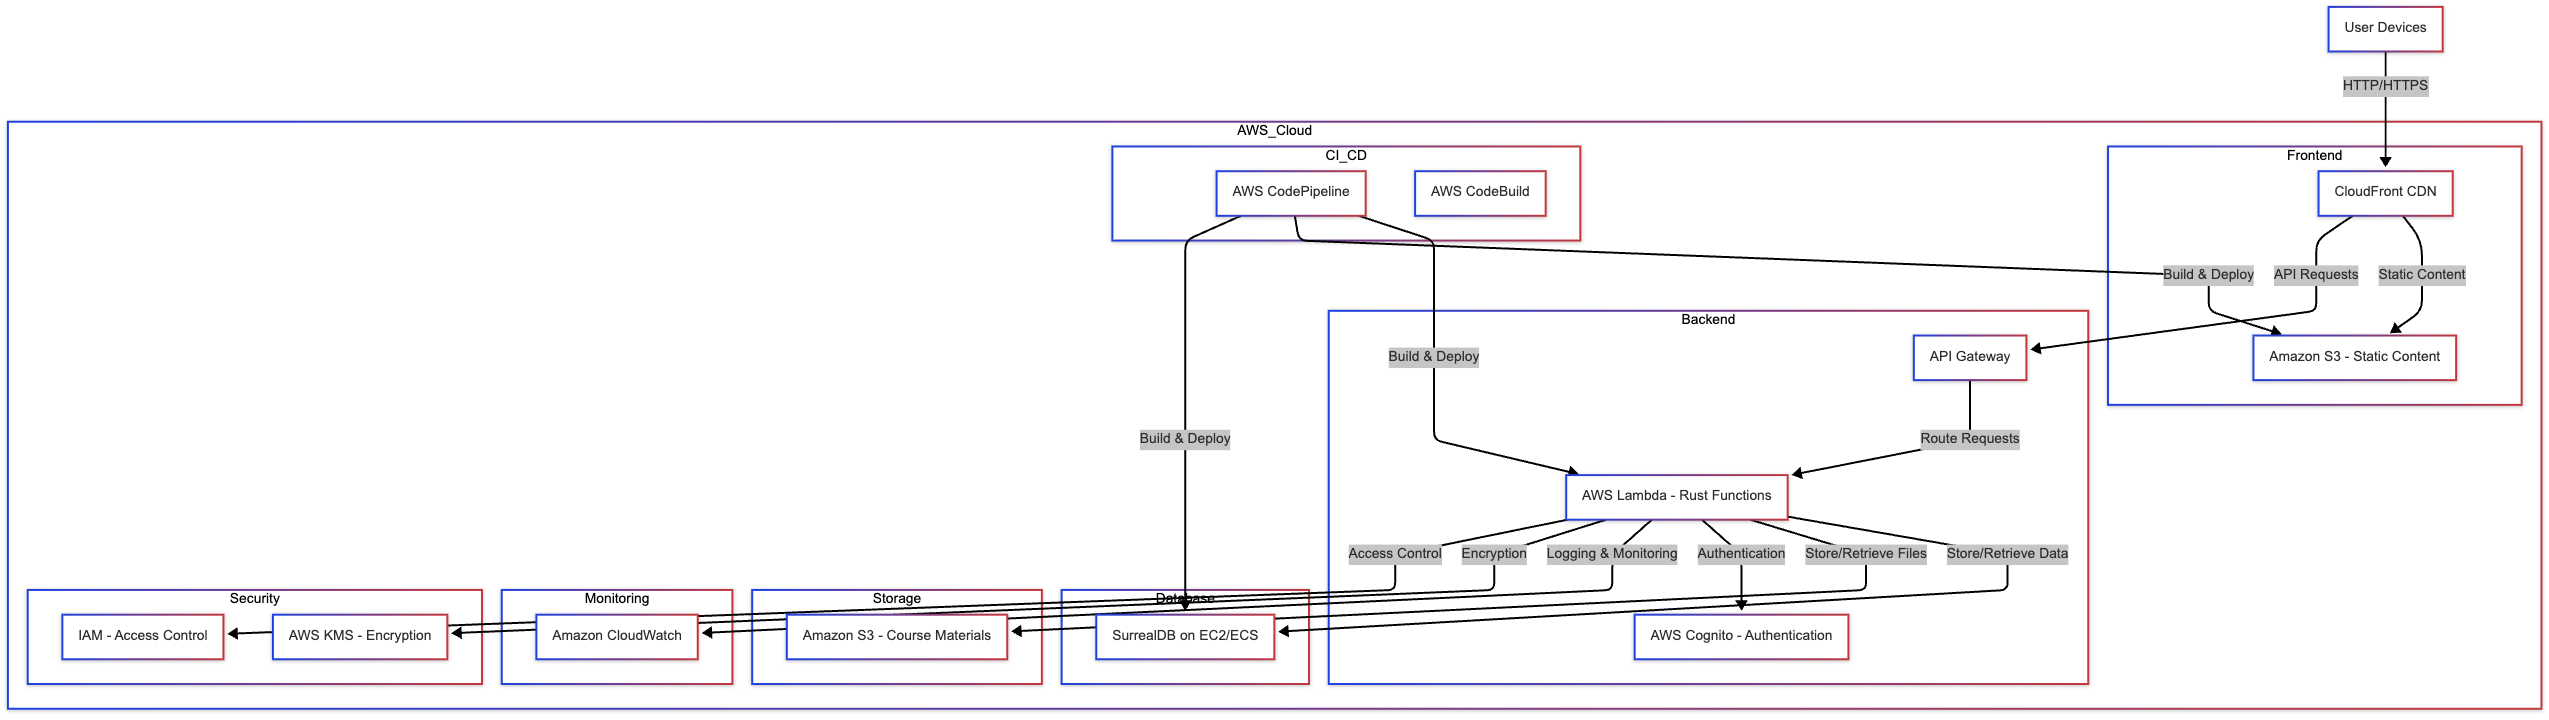
\includegraphics[width=0.5\textwidth]{serverless_deployment.png}
    \caption{AWS Serverless Deployment Architecture}
\end{figure}

Key interactions between components include:
\begin{itemize}
    \item Users access the system via web browsers or mobile devices, connecting to CloudFront CDN
    \item CloudFront delivers static content from S3 and routes API requests to API Gateway
    \item API Gateway manages all external requests and routes them to appropriate Lambda functions
    \item Lambda functions (built in Rust) handle business logic, interacting with SurrealDB for data storage
    \item AWS Cognito manages authentication and user identity before business logic executes
    \item Lambda functions use S3 for file storage and SNS for notifications
    \item CloudWatch provides logging and monitoring capabilities
    \item KMS and IAM handle encryption and access control respectively
    \item CI/CD pipeline with CodePipeline and CodeBuild automates deployment
\end{itemize}

\section{Database}
The database architecture of Kaiju Academy is built on SurrealDB, a multi-model database that provides flexibility in data modeling.
It is hosted on AWS as a Infrastructure-as-a-Service (IaaS) using AWS EC2 for high availability and scalability, it facilitates the integration with other AWS services like Lambda, API Gateway, S3 etc. with
increased efficiency and performance.

\section{Security}
\subsection{Infrastructure Security}
As our application is deployed on AWS as a Platform-as-a-Service (PaaS) using Lambda functions, the majority of infrastructure security is managed by AWS. We leverage the following AWS-managed security features:

\begin{itemize}
    \item \textbf{Network Security:}
    \begin{itemize}
        \item AWS-managed VPC isolation for Lambda functions
        \item Built-in AWS Shield protection against DDoS attacks
        \item AWS-configured security boundaries between services
    \end{itemize}
    
    \item \textbf{Data Security:}
    \begin{itemize}
        \item AWS-managed AES-256 encryption at rest
        \item AWS-enforced TLS 1.2+ for data in transit
        \item Automated key management through AWS KMS
    \end{itemize}
\end{itemize}

\subsection{Application Security}
\begin{itemize}
    \item \textbf{Input Validation:}
    \begin{itemize}
        \item Request validation at API Gateway
        \item Sanitization of user inputs
        \item Rate limiting per user/IP
    \end{itemize}
    
    \item \textbf{Code Execution Security:}
    \begin{itemize}
        \item Dockerized isolated environments for isolated user code execution:
        \begin{itemize}
            \item Leverage AWS Fargate to run containers without server management.
            \item Ensure secure, scalable, and efficient execution of user-submitted code.
            \item Package each user code submission into a Docker container.
            \item Encapsulate dependencies and runtime configurations within the container.
            \item Enable AWS Lambda to trigger these containers for seamless integration.
            \item Maintain isolation and resource limits for each execution.
        \end{itemize}
        \item Our Lambda handling functions are built on Rust, which provides:
        \begin{itemize}
            \item Memory safety through its ownership model, preventing data races and ensuring safe memory access.
            \item Compile-time checks that catch potential errors before deployment, reducing runtime vulnerabilities.
            \item Strict borrowing rules that enforce safe access patterns, minimizing the risk of buffer overflows.
            \item A strong type system that helps prevent injection attacks by ensuring that data types are correctly handled.
            \item Fast execution speed without sacrificing safety, enabling rapid processing of user-submitted code.
        \end{itemize}
    \end{itemize}
\end{itemize}

\section{User Authentication and Authorization}
\subsection{Authentication Flow with AWS Cognito}
\begin{itemize}
    \item \textbf{User Registration:}
    \begin{itemize}
        \item Cognito User Pools for email/password and social identity providers
        \item Automated email verification workflows
        \item Built-in MFA options (SMS, TOTP authenticator apps)
    \end{itemize}
    
    \item \textbf{Session Management:}
    \begin{itemize}
        \item Cognito-issued JWT tokens (ID, Access, and Refresh tokens)
        \item Token validation via Cognito's public keys
        \item Configurable token expiration policies
    \end{itemize}
\end{itemize}

\subsection{Authorization Model with AWS IAM}
\begin{itemize}
    \item \textbf{Role-Based Access Control:}
    \begin{itemize}
        \item IAM roles mapped to Cognito user groups (Student, Educator, Admin)
        \item Fine-grained IAM policies for service access
        \item Temporary credentials via Cognito Identity Pools
    \end{itemize}
    
    \item \textbf{Integration Points:}
    \begin{itemize}
        \item Cognito authorizers for API Gateway endpoints
        \item Resource-based policies for Lambda functions
        \item IAM-based access control for AWS services (S3, DynamoDB)
    \end{itemize}
\end{itemize}

\section{Content Delivery}
The content delivery infrastructure is built on AWS CloudFront CDN and S3, optimized for global distribution of both static and dynamic content.

\section{Testability}

\subsection{Automated Testing}
With the benefits of Rust's built-in support for a robust testing system, our app can undergo rigorous testing in the pipeline automatically. This automation ensures that every code change is validated through a series of tests, significantly enhancing the reliability and functionality of the application.

\subsection{Types of Tests}
Rust's testing framework allows for various types of tests, including:
\begin{itemize}
    \item \textbf{Unit Tests:} These tests validate individual components or functions, ensuring that each part of the code behaves as expected in isolation.
    \item \textbf{Integration Tests:} These tests assess the interactions between different components, verifying that they work together correctly and that the overall system functions as intended.
    \item \textbf{Documentation Tests:} Rust allows for tests to be embedded within documentation comments, ensuring that examples remain accurate and functional as the code evolves.
\end{itemize}

\subsection{Continuous Integration}
By integrating automated testing into our continuous integration/continuous deployment (CI/CD) pipeline, we can ensure that every code change is thoroughly tested before deployment. This practice helps identify issues early in the development cycle, reducing the risk of bugs in production and maintaining high standards of quality and performance throughout the development process.

\chapter{Data Models}

\section{Database Schema}
The database design incorporates relational, document, and graph capabilities through SurrealDB's multi-model approach.

\begin{figure}[!ht]
    \centering
    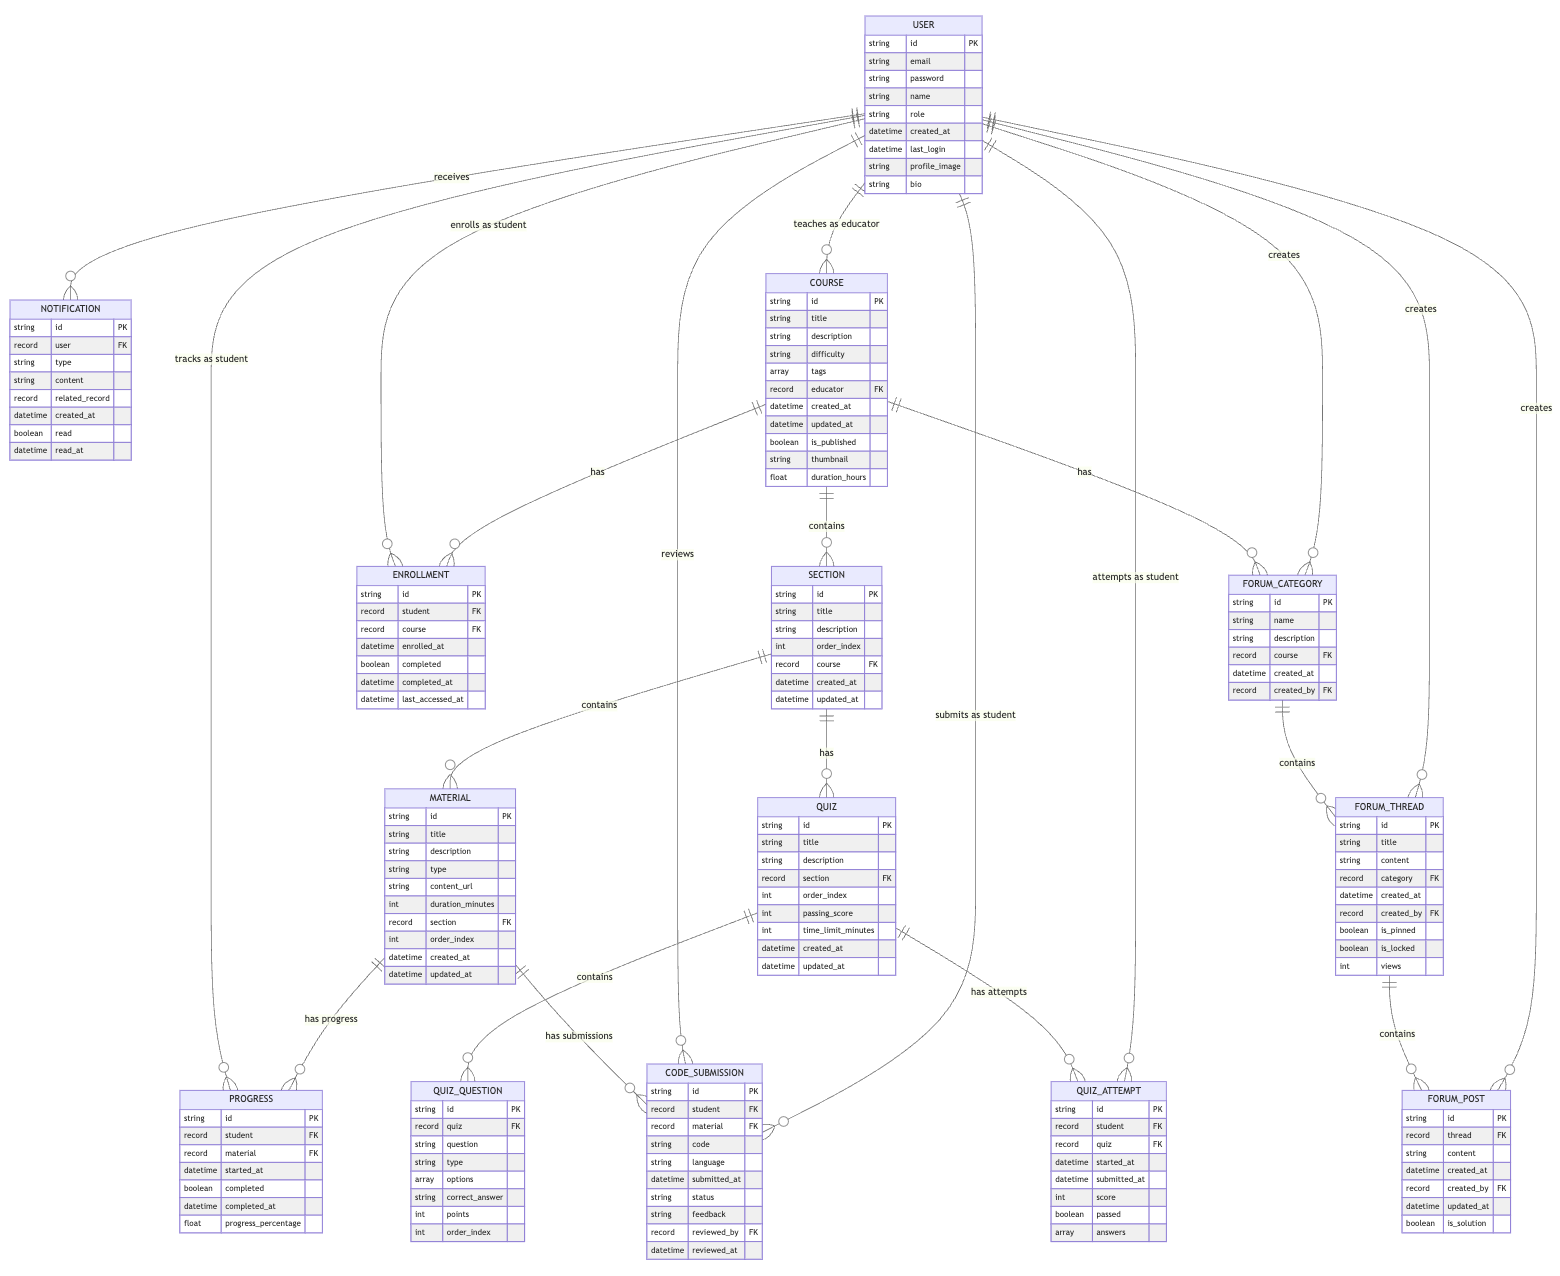
\includegraphics[width=\textwidth]{database_schema.png}
    \caption{Database Schema}
\end{figure}

\section{Request and Response Structure}
AWS Lambda functions are event-driven, the request and response structure is defined in the Lambda function code. And in Rust SDK, the 
request and response structure is defined as
\begin{enumerate}
    \item \texttt{LambdaEvent<ApiGatewayProxyRequest>}
    \item \texttt{Result<ApiGatewayProxyResponse, Error>}
\end{enumerate}
And it is an example of how we structure the response in the function handler:
\begin{lstlisting}[language=Rust]
    // other handler body code
    let response = ApiGatewayProxyResponse { // define response object
        status_code: 200,
        headers: std::collections::HashMap::new(),
        multi_value_headers: std::collections::HashMap::new(),
        body: Some(json!({ "message": "Hello from Kaiju Academy API!" }).to_string()),
        is_base64_encoded: Some(false),
    };
    Ok(response) // return the response as Option::Ok
\end{lstlisting}

\section{Data Flow Sequence}
The following diagram illustrates the flow of data through the system:

\begin{figure}[ht]
    \centering
    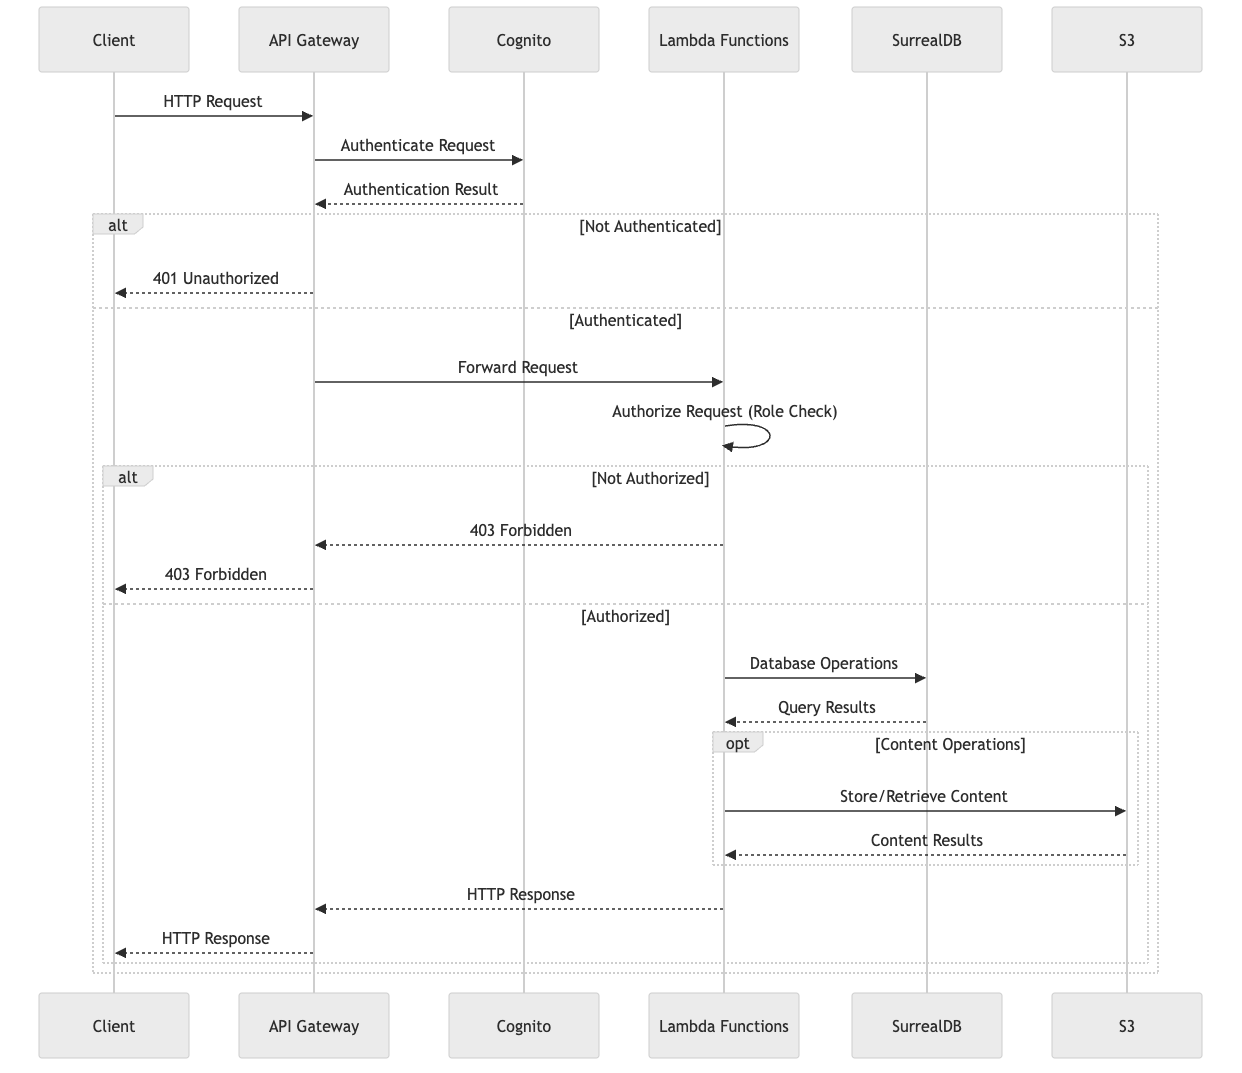
\includegraphics[width=\textwidth]{data_flow.png}
    \caption{Data Flow Sequence Diagram}
\end{figure}

\chapter{Interface Design}

\section{User Registration and Authentication}
\begin{figure}[!htb]
    \centering
    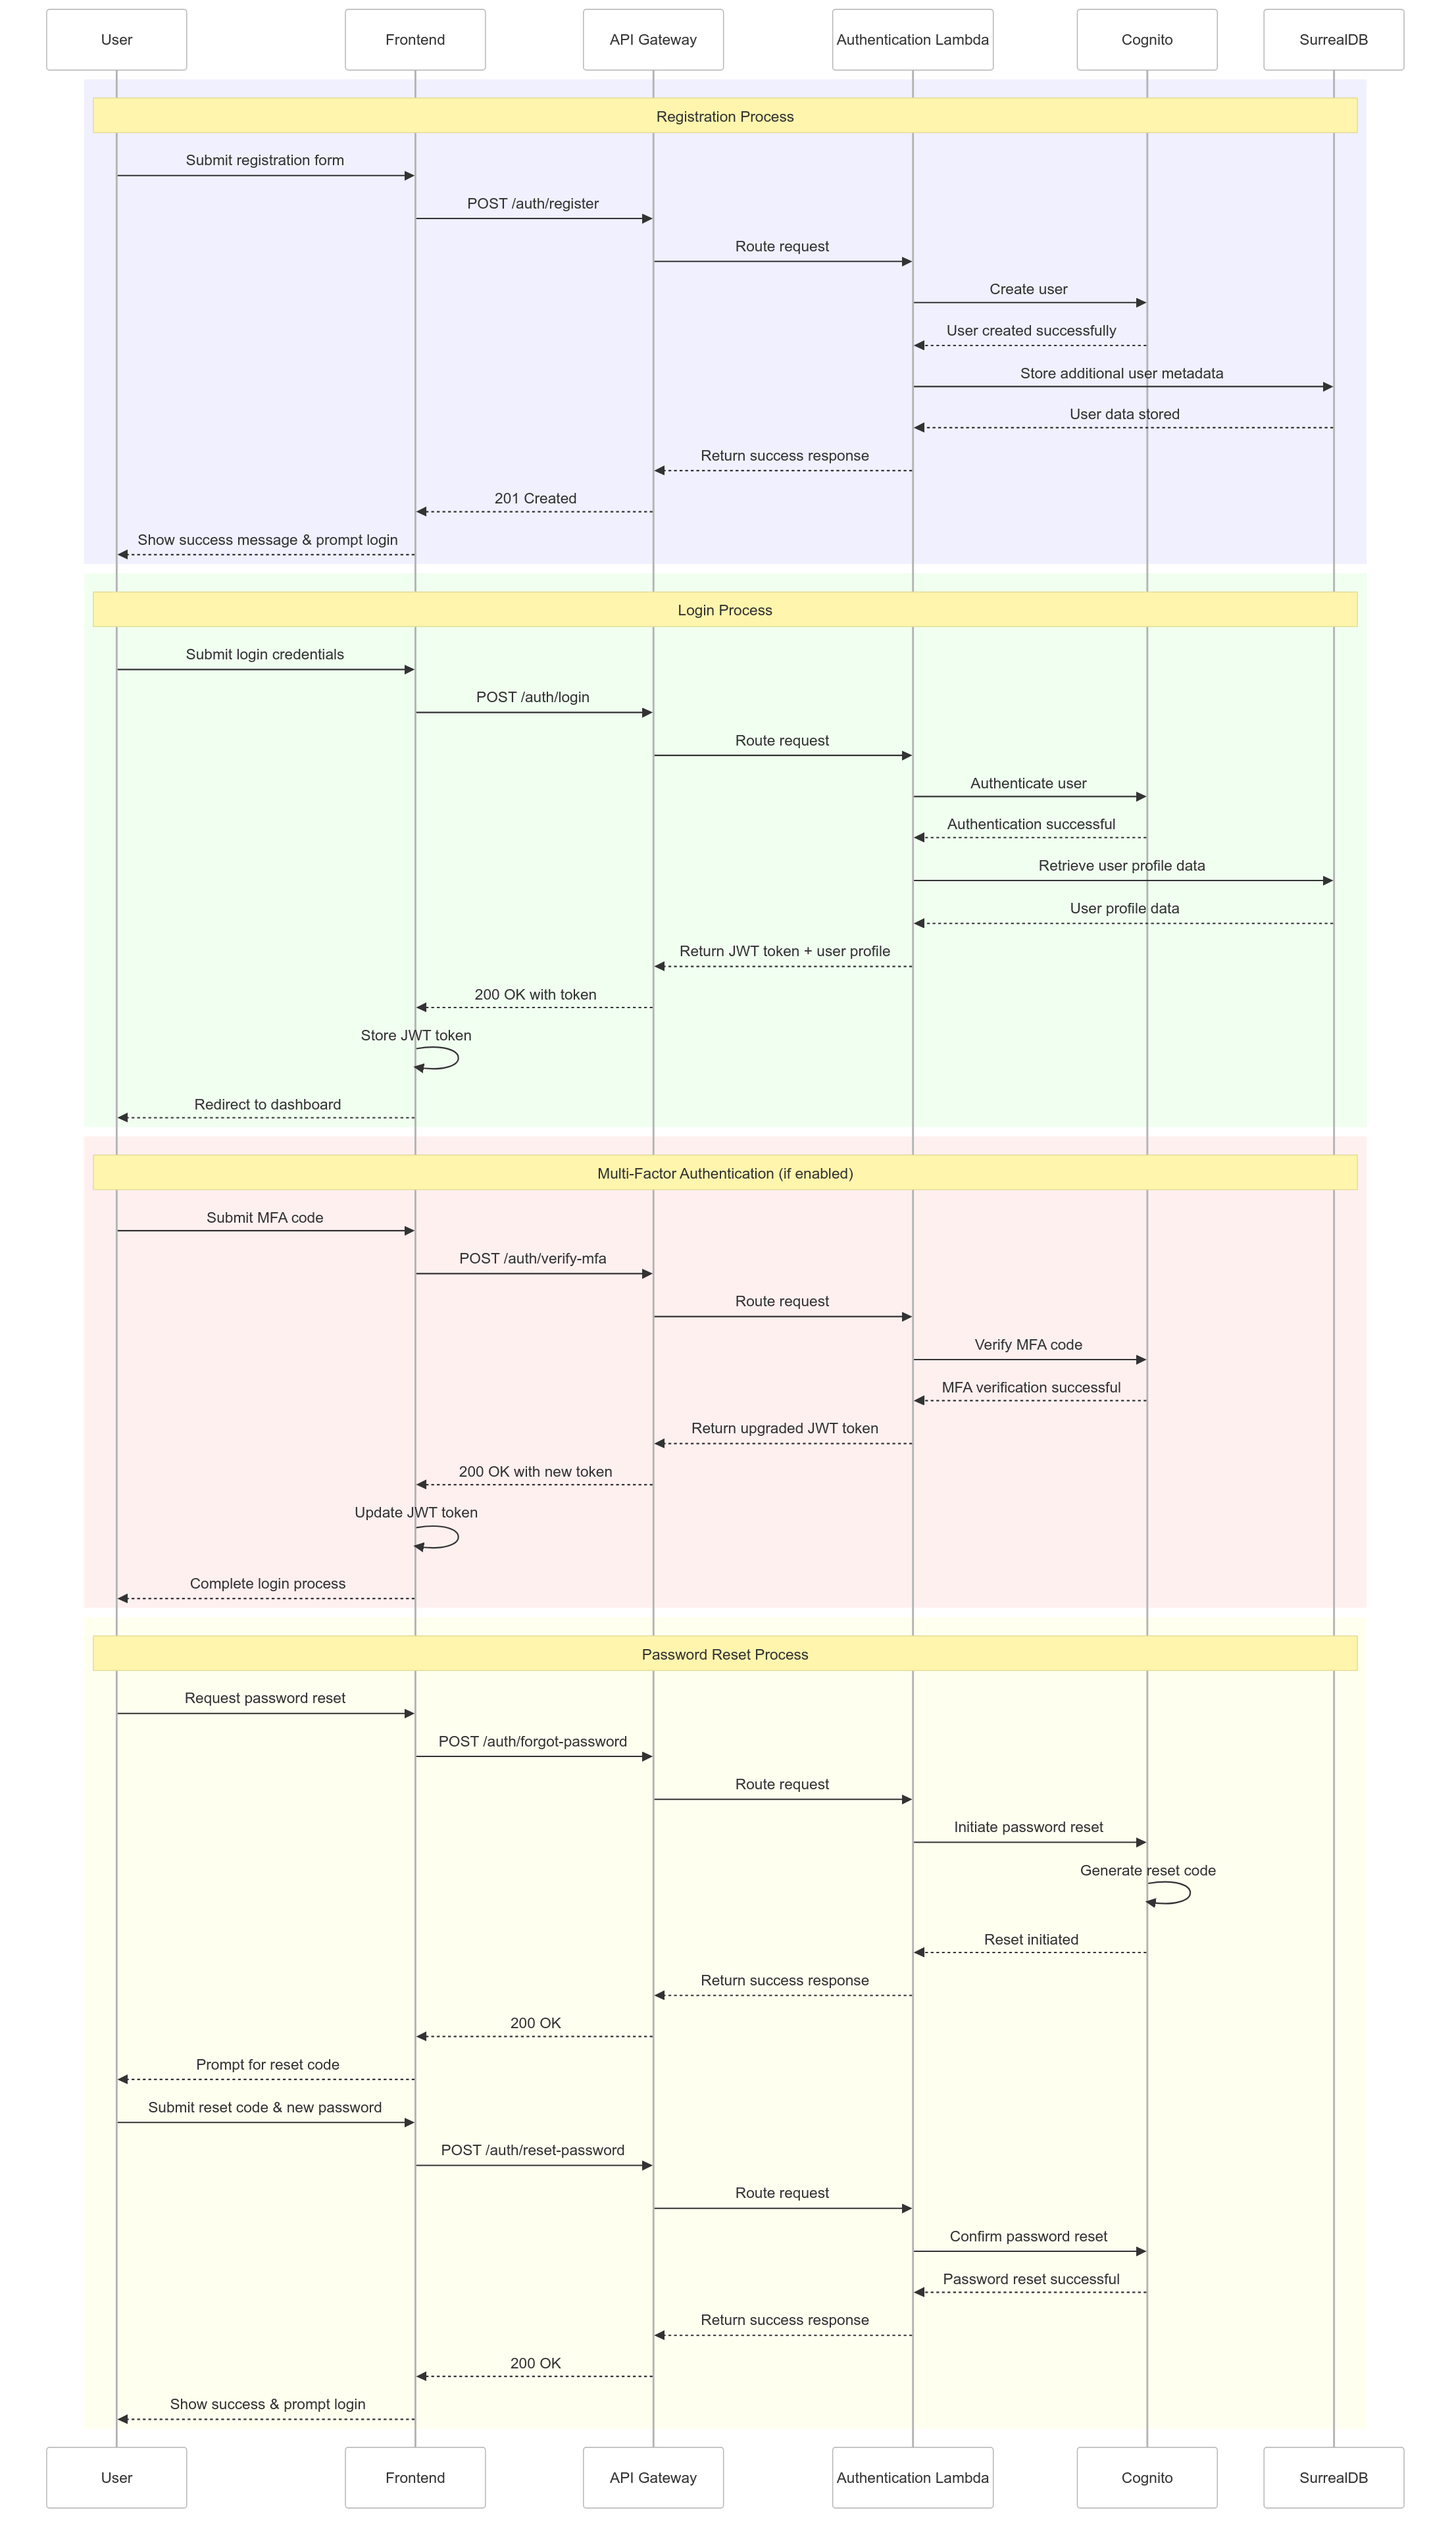
\includegraphics[height=0.7\textheight]{user_authentication.png}
    \caption{User Authentication Workflow}
\end{figure}

\begin{enumerate}
    \item User submits registration data through frontend
    \item API Gateway routes to Authentication Lambda
    \item Lambda creates user in Cognito and SurrealDB
    \item JWT token returned for authenticated session
\end{enumerate}

\subsection{Course Management}

\subsubsection{Course Content Management}
\begin{figure}[!htb]
    \centering
    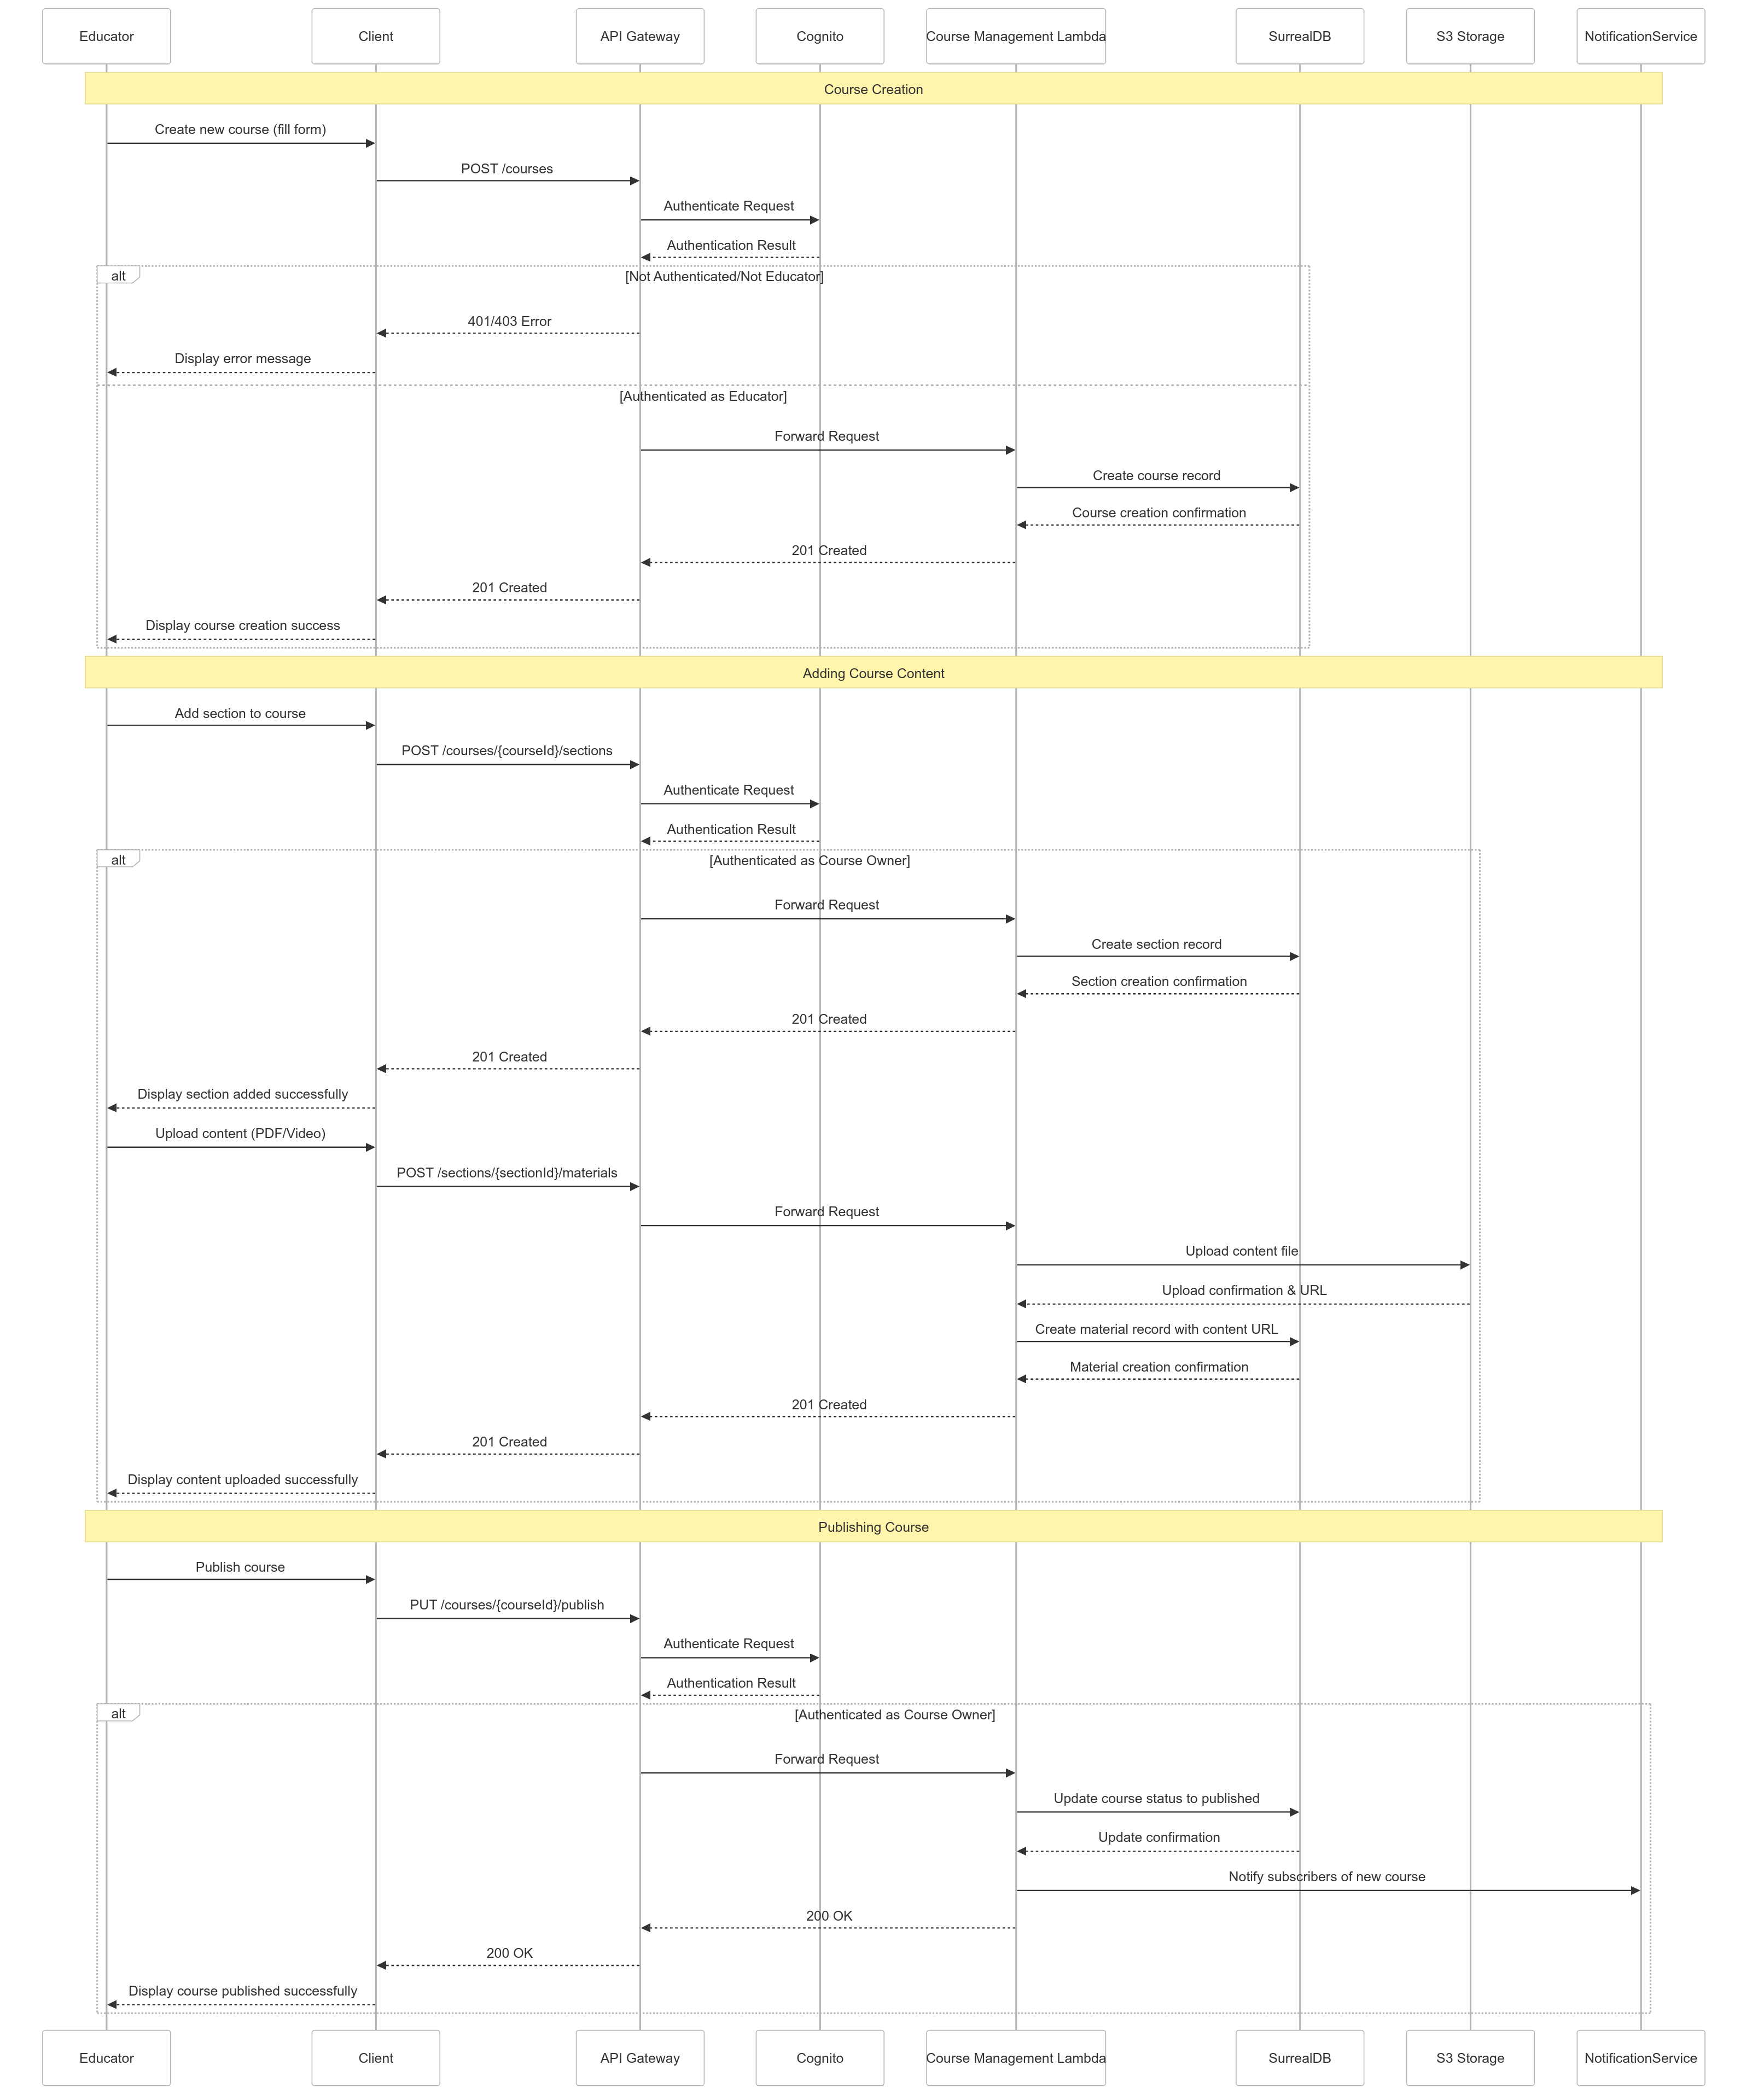
\includegraphics[height=0.75\textheight]{educator_managing_courses.png}
    % TODO: Convert mermaid diagram to PNG or update path to existing diagram
    \caption{Course Management Workflow}
\end{figure}


\begin{enumerate}
    \item Educator creates course structure through UI
    \item Course metadata and structure stored in SurrealDB
    \item Materials uploaded to S3 with references stored in database
    \item Publishing workflow updates visibility and notifies subscribers
\end{enumerate}

\subsection{Course Access}
\begin{figure}[!htb]
    \centering
    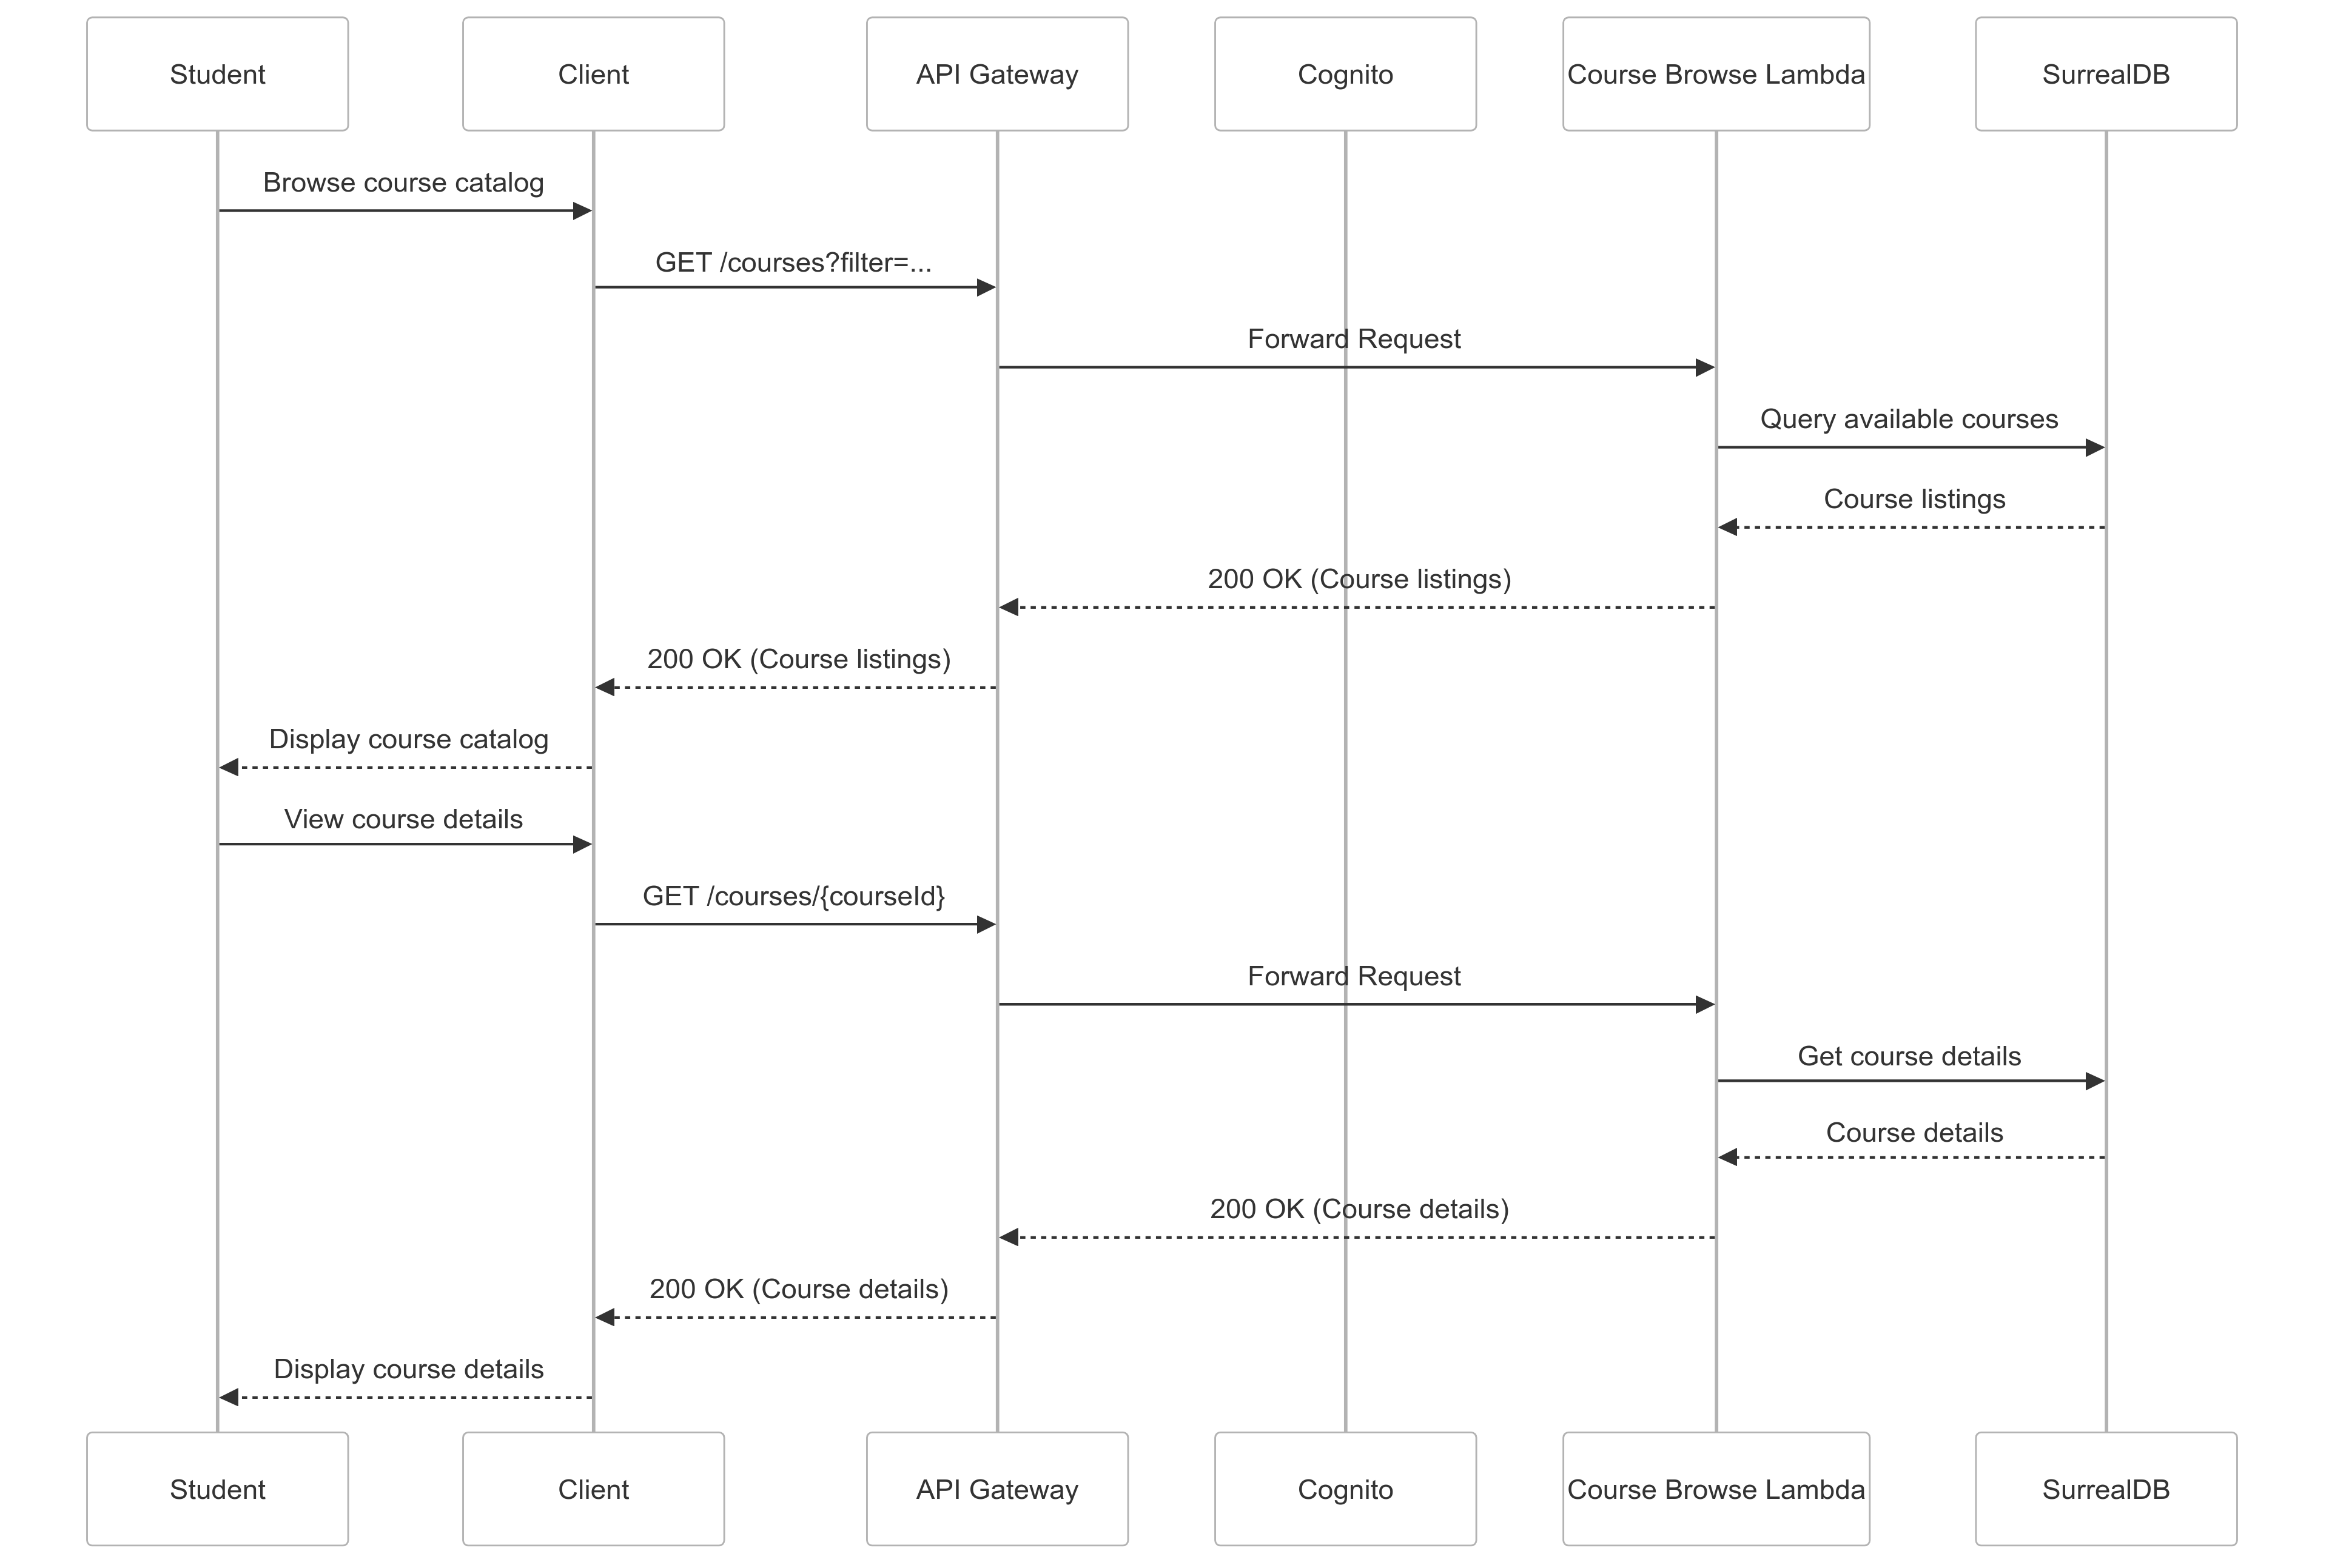
\includegraphics[height=0.4\textheight]{student_access_course.png}
    % TODO: Convert mermaid diagram to PNG or update path to existing diagram
    \caption{Course Access Workflow}
\end{figure}

\subsection{Code Assessment and Grading}
\begin{figure}[!htb]
    \centering
    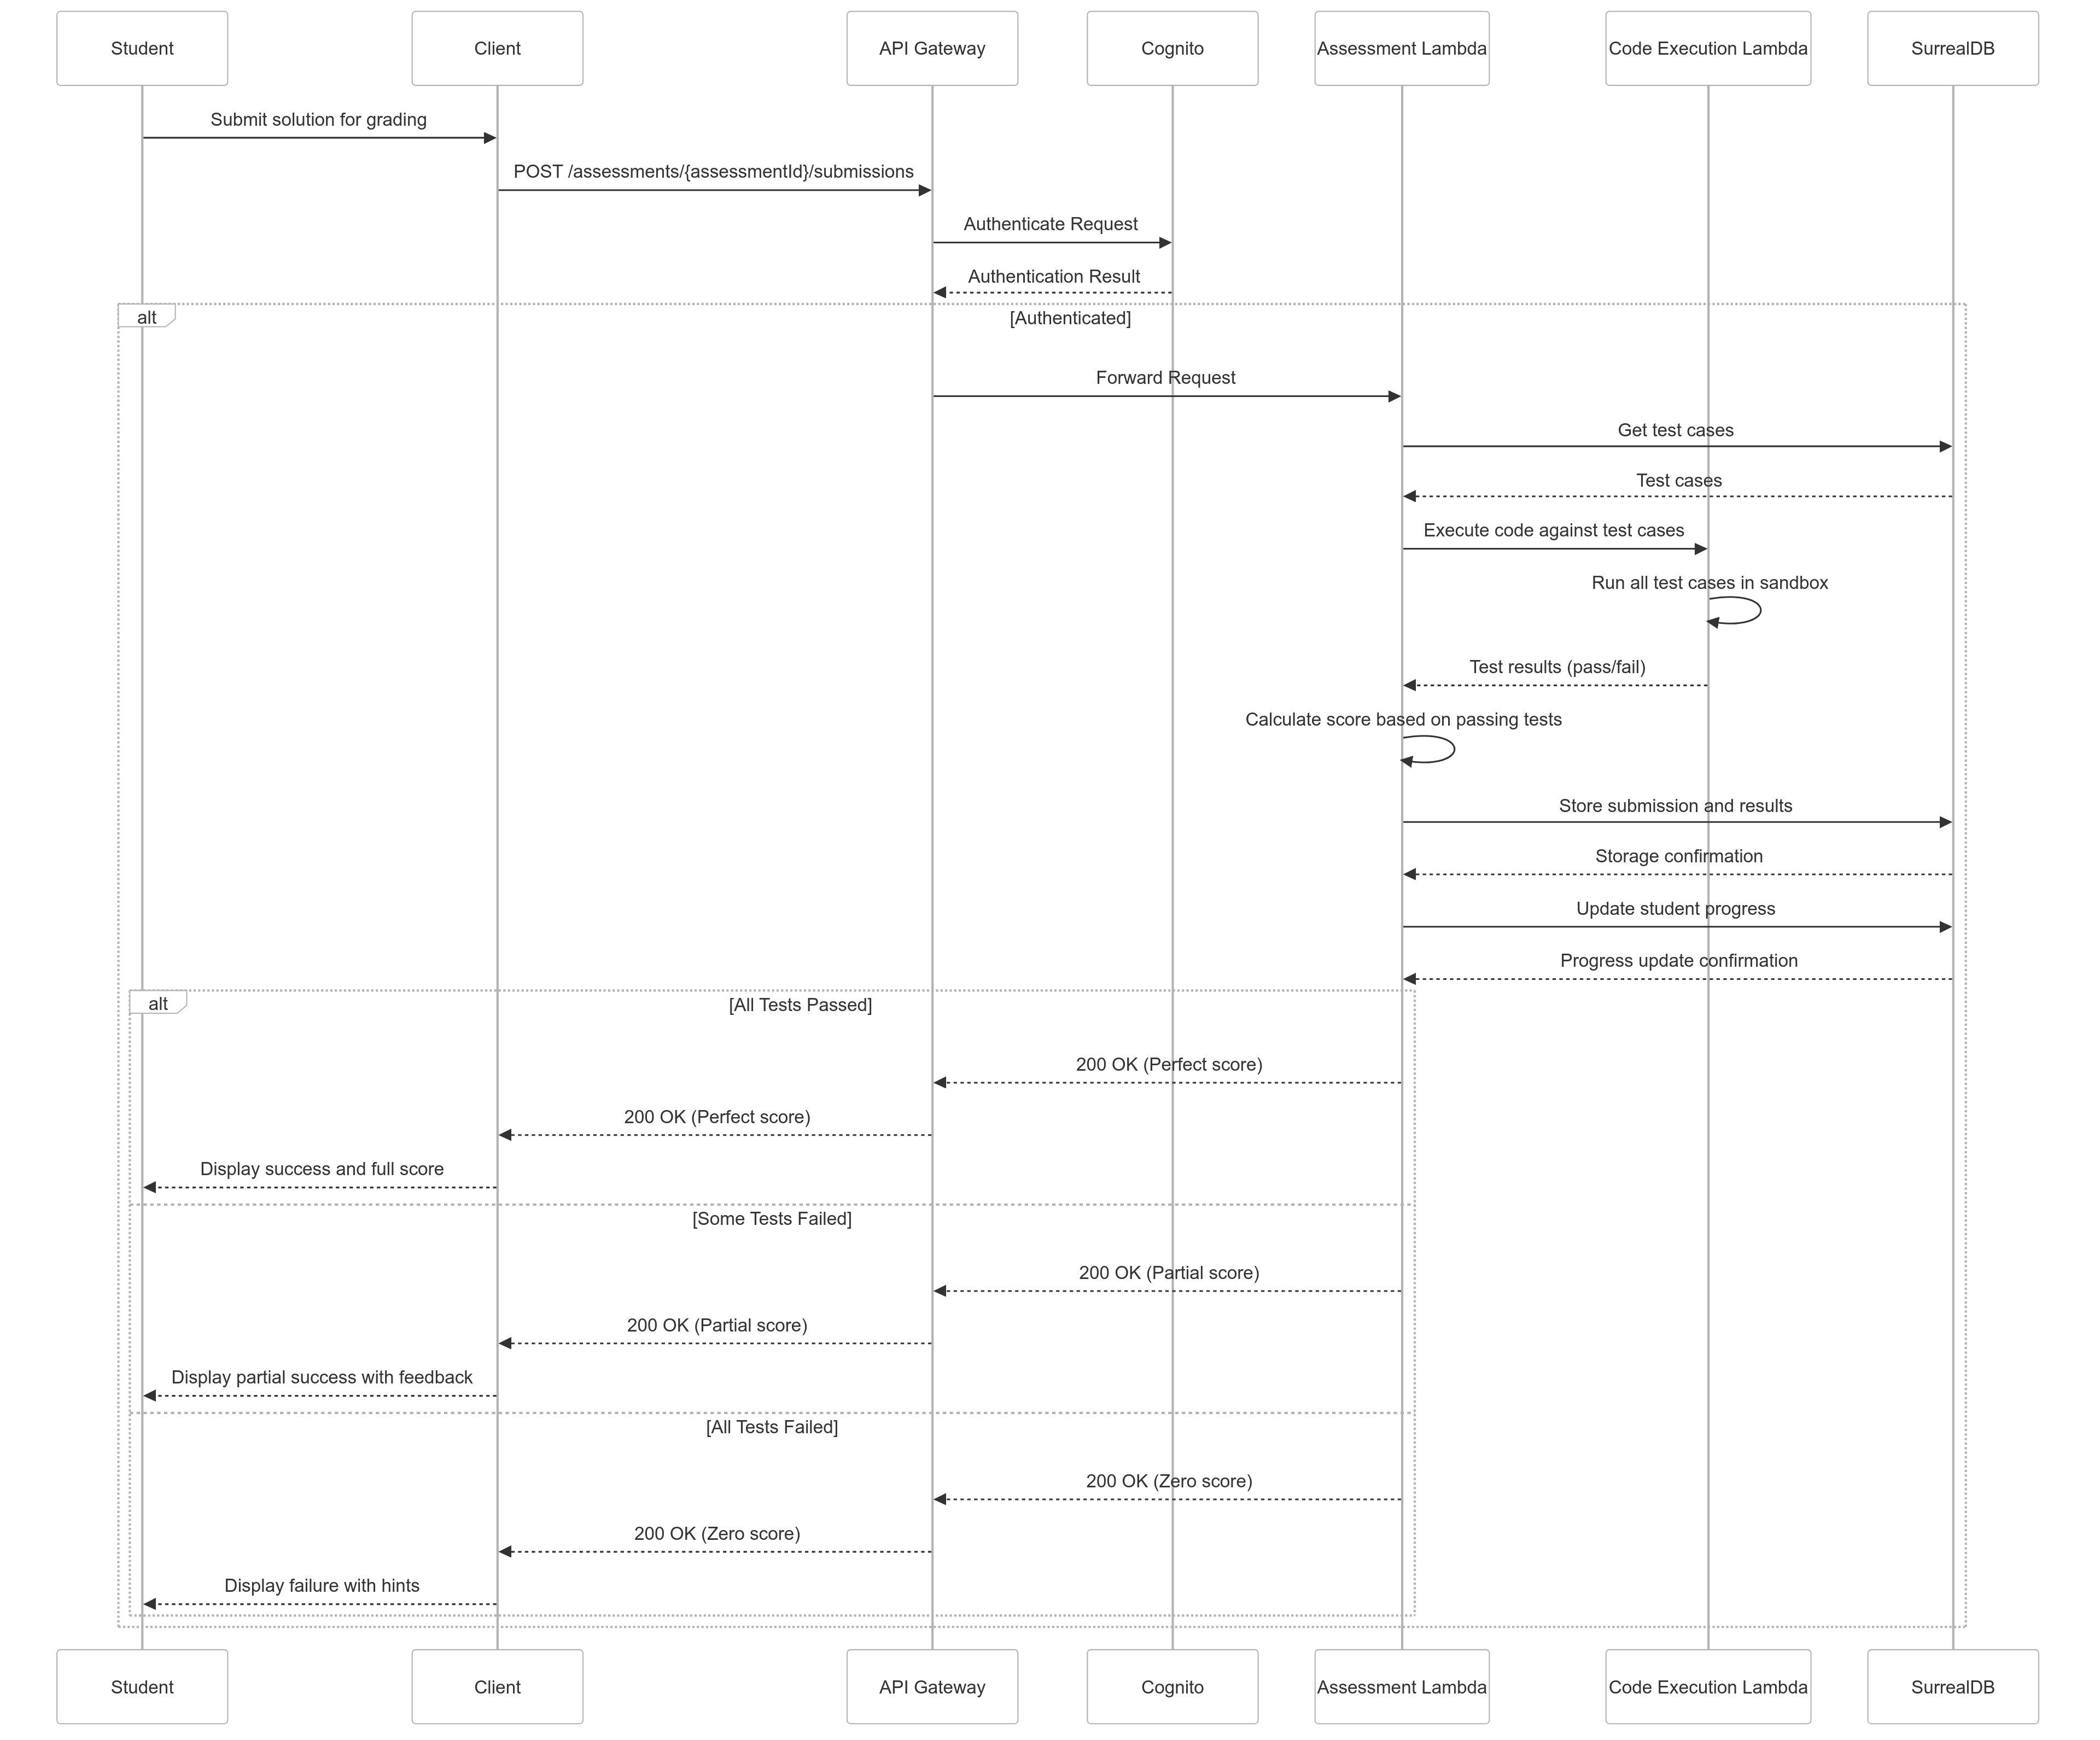
\includegraphics[height=0.4\textheight]{code_grade.png}
    % TODO: Convert mermaid diagram to PNG or update path to existing diagram
    \caption{Code Auto-grading Workflow}
\end{figure}


\subsection{Forum Moderation}
\begin{figure}[!htb]
    \centering
    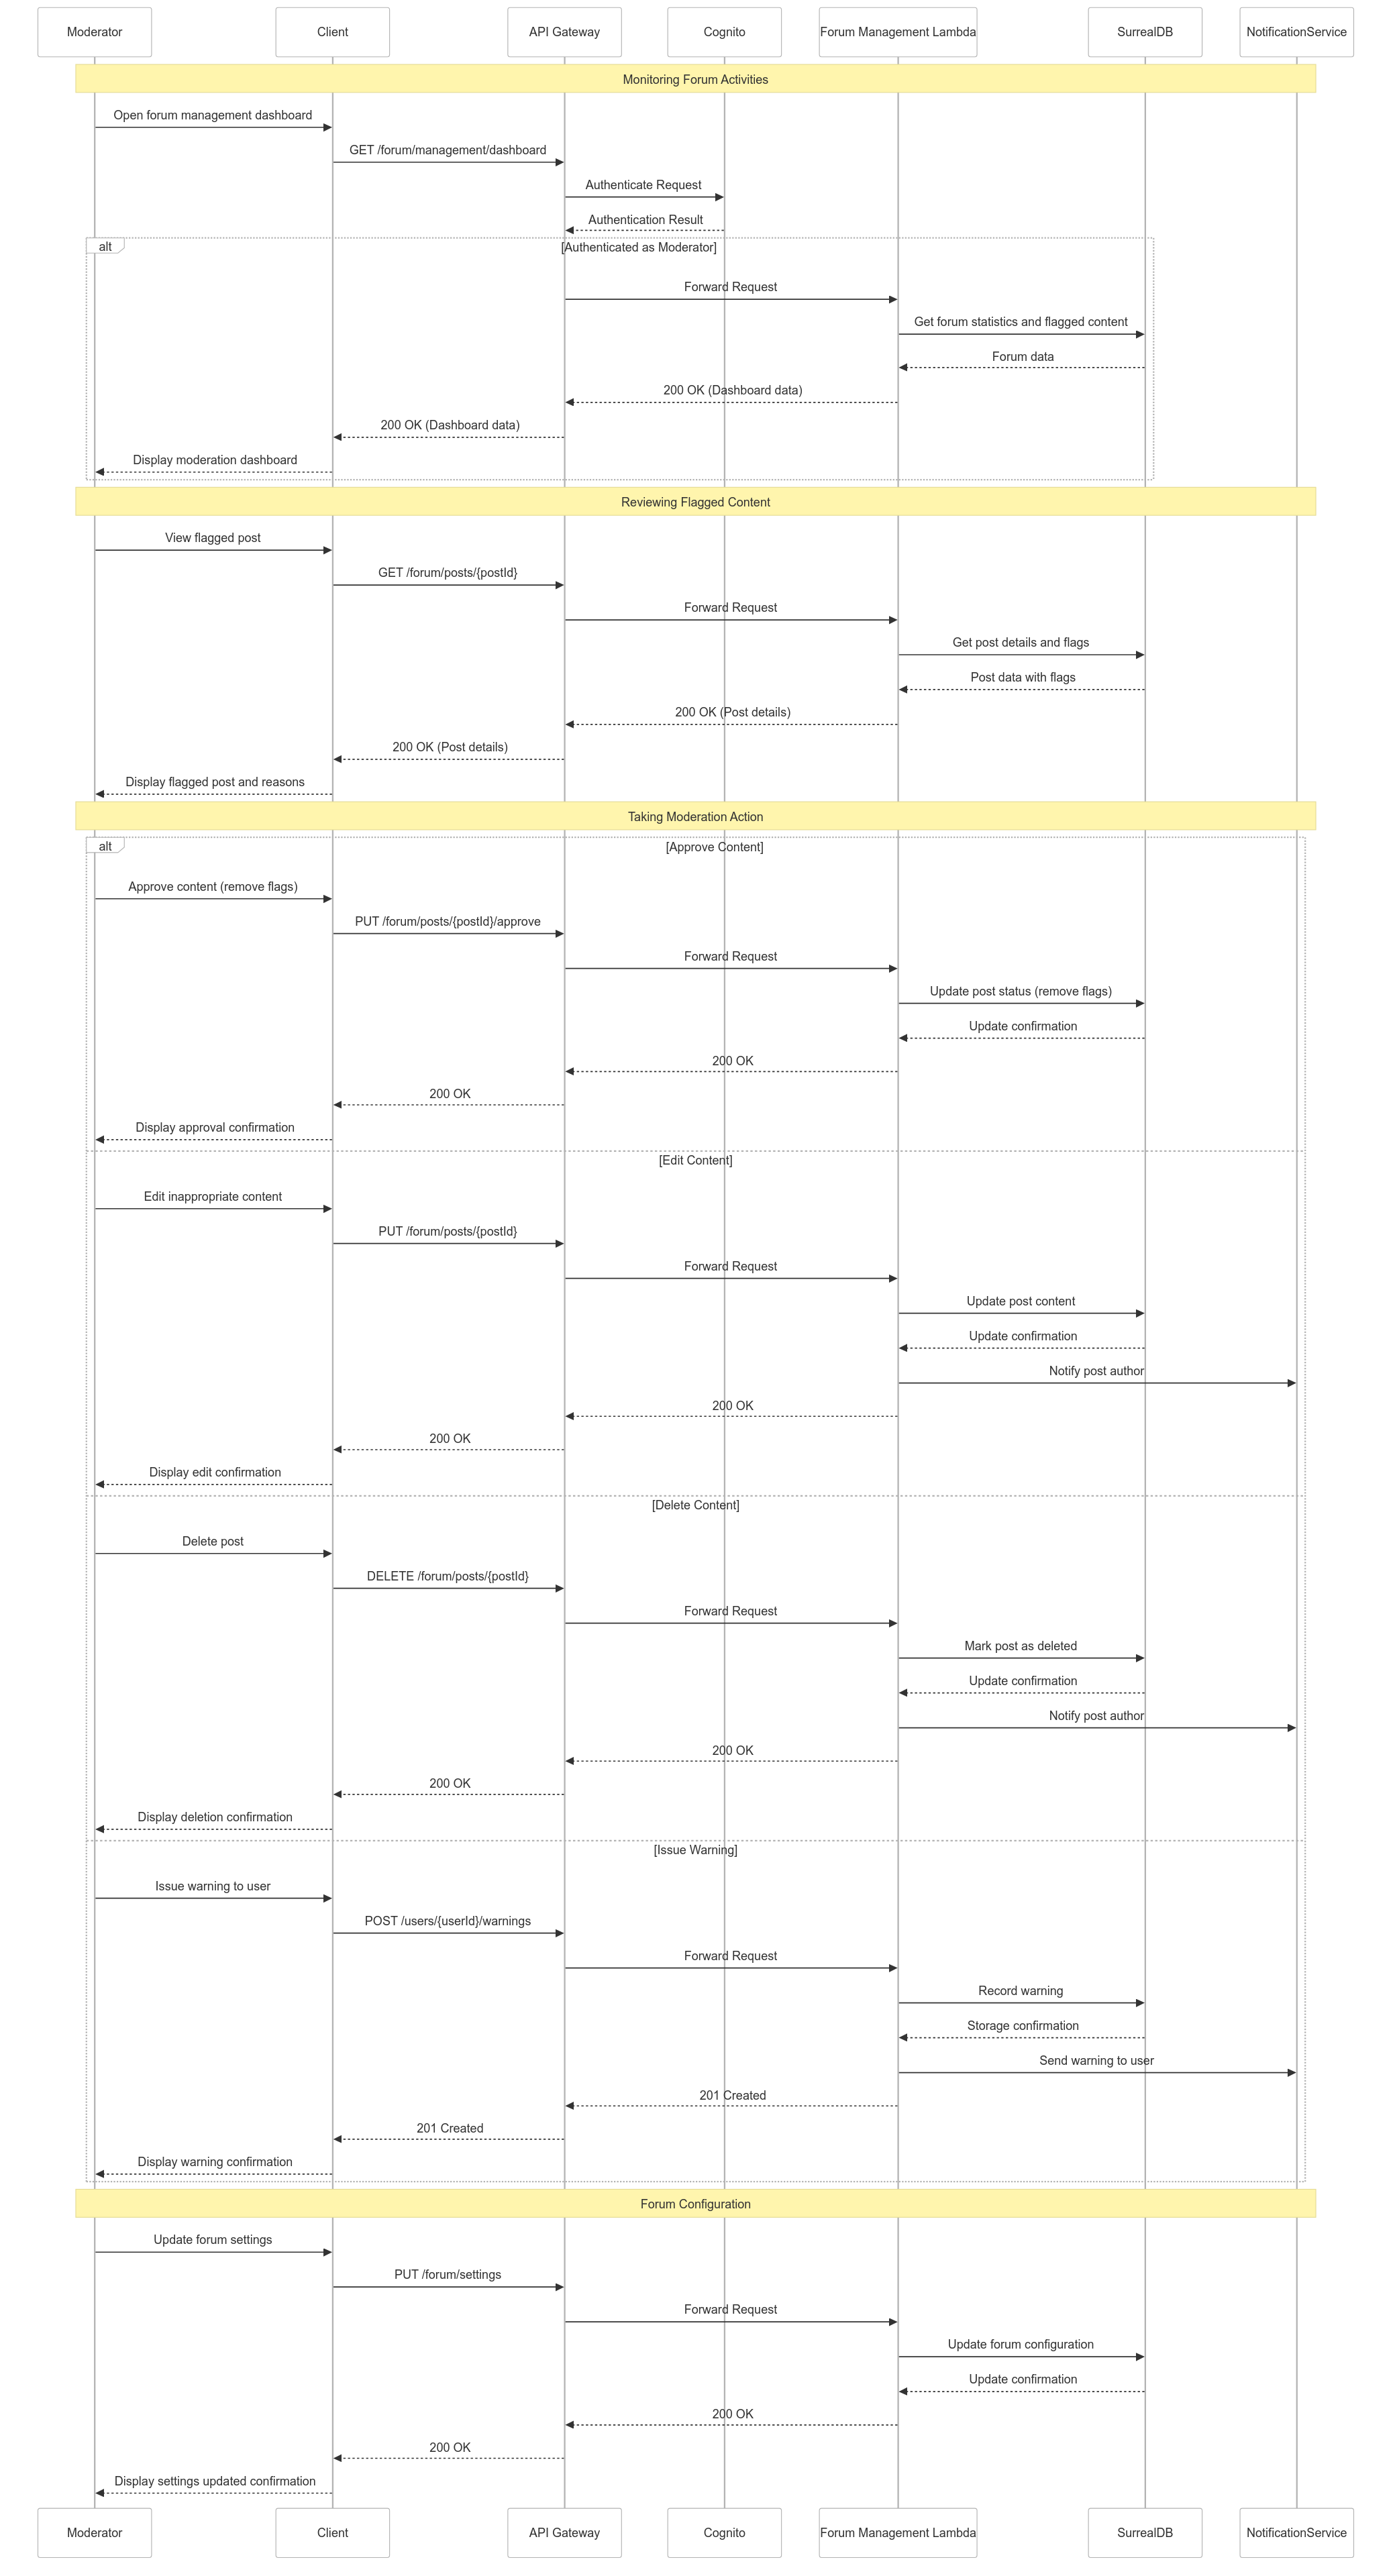
\includegraphics[height=0.9\textheight]{moderator_managing_forum.png}
    \caption{Moderator Managing Forum Process}
\end{figure}

% \section{API Structure}
% The API follows RESTful principles organized into domain-specific endpoints. All external communication occurs through a standardized API Gateway.
% TODO: Add API structure diagram

\section{Service Communication}

\subsection{External Interfaces}
\begin{itemize}
    \item RESTful APIs with JSON payloads
    \item Rate limiting (10 requests/second per user)
    \item Batch operations for efficiency
    \item Pagination for large result sets
\end{itemize}

\subsection{Internal Communication}
\begin{itemize}
    \item AWS SNS/SQS for asynchronous event processing
    \item AWS Step Functions for complex workflows
    \item Direct Lambda invocations for synchronous operations
\end{itemize}

\section{Security Implementation}
\begin{figure}[ht]
    \centering
    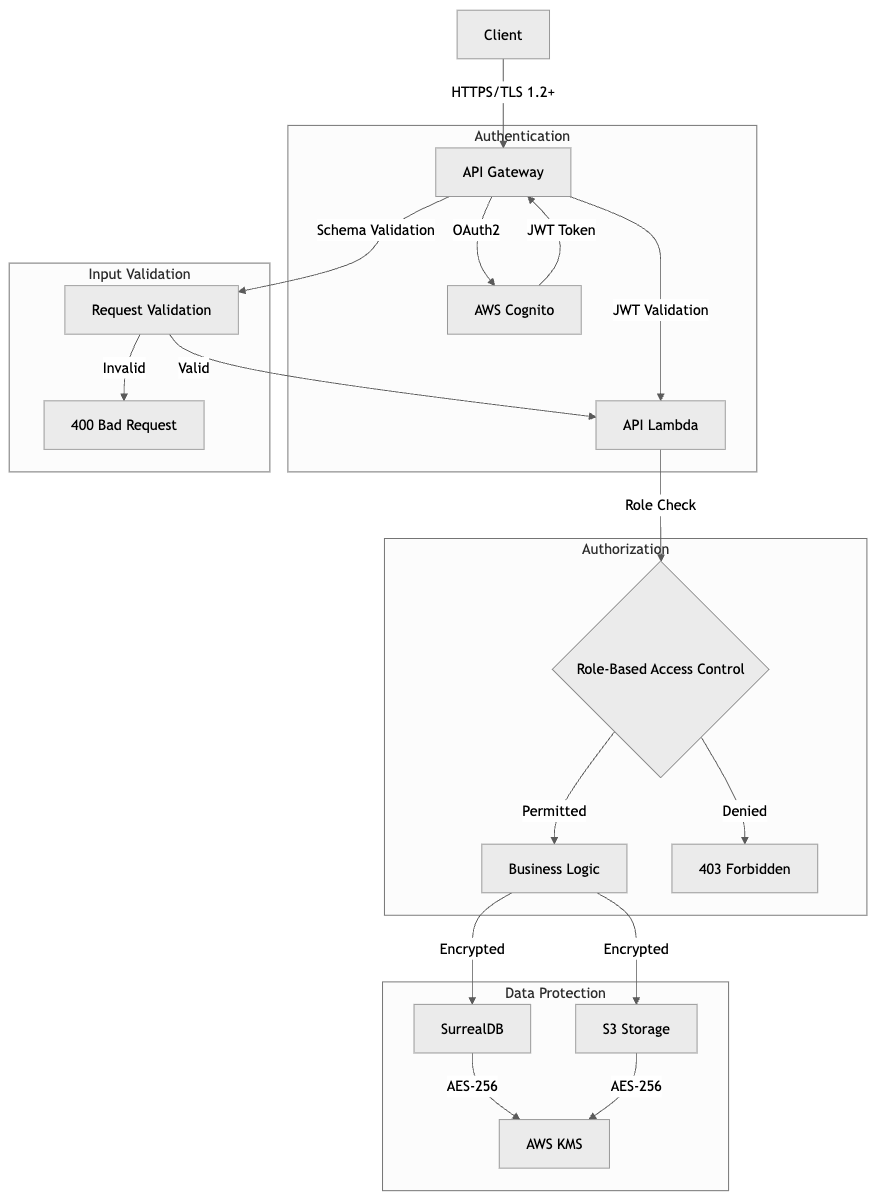
\includegraphics[height=0.6\textheight]{security_implementation.png}
    \caption{Security Implementation Diagram}
\end{figure}

\subsection{Authentication and Authorization}
\begin{itemize}
    \item Multi-factor Authentication (MFA): Optional for all users, required for administrators
    \item OAuth2 Integration: Support for Google, GitHub, and Microsoft accounts
    \item Role-based Access Control (RBAC): Granular permissions based on user roles
    \item JWT for API Authentication: Secure, stateless authentication for API requests
\end{itemize}

\subsection{Data Protection}
\begin{itemize}
    \item Encryption at Rest: AES-256 encryption for all sensitive data
    \item Encryption in Transit: TLS 1.2+ for all network communications
    \item PII Protection: Minimized collection of personally identifiable information
    \item Data Retention Policies: Automated purging of unnecessary data
\end{itemize}

\section{Exception Handling}

\subsection{Expected Exceptions}
We followed the standardized error model in the API Gateway and Lambda functions, expected the following error types:\\
\begin{itemize}
    \item Authentication errors (401) 
        \begin{description}
            \item[Possible causes:] Invalid username/password combinations or expired authentication tokens.
            \item[Raise:] 401 Unauthorized
        \end{description}
    \item Authorization errors (403) 
        \begin{description}
            \item[Possible causes:] Insufficient user permissions or attempts to access restricted resources.
            \item[Raise:] 403 Forbidden
        \end{description}
    \item Validation errors (400) 
        \begin{description}
            \item[Possible causes:] Malformed input data, missing required fields, or invalid data formats.
            \item[Raise:] 400 Bad Request
        \end{description}
    \item Not found errors (404) 
        \begin{description}
            \item[Possible causes:] Requests for non-existent endpoints or resources that have been deleted or never existed.
            \item[Raise:] 404 Not Found
        \end{description}
    \item Database errors (500) 
        \begin{description}
            \item[Possible causes:] Query syntax errors, connection timeouts, or database server outages.
            \item[Raise:] 500 Internal Server Error
        \end{description}
    \item Internal server errors (500) 
        \begin{description}
            \item[Possible causes:] Unhandled exceptions, misconfigurations, or resource exhaustion within the application.
            \item[Raise:] 500 Internal Server Error
        \end{description}
    \item External service errors (502) 
        \begin{description}
            \item[Possible causes:] Network issues, timeouts, or unavailability of downstream services.
            \item[Raise:] 502 Bad Gateway
        \end{description}
    \item Rate limit errors (429) 
        \begin{description}
            \item[Possible causes:] Exceeding the allowed number of requests in a specified time frame due to aggressive client behavior.
            \item[Raise:] 429 Too Many Requests
        \end{description}
\end{itemize}


\subsection{Error Triggering Mechanisms}
\begin{itemize}
    \item \textbf{API Request Validation:}
    \begin{itemize}
        \item Automatic schema validation at API Gateway
        \item Input parameter validation in Lambda functions
        \item Business logic validation in service layer
    \end{itemize}
    
    \item \textbf{Security Checks:}
    \begin{itemize}
        \item JWT token validation
        \item Permission verification against IAM policies
        \item Resource ownership verification
    \end{itemize}
    
    \item \textbf{External Integrations:}
    \begin{itemize}
        \item Timeout detection for external services
        \item Error propagation from downstream systems
        \item Network failure detection
    \end{itemize}
\end{itemize}

\subsection{Error Handling Strategy}
\begin{itemize}
    \item \textbf{Error Processing Flow:}
    \begin{itemize}
        \item Error detection at appropriate layer
        \item Conversion to standard AppError type
        \item Automatic mapping to API Gateway responses
        \item Logging with correlation IDs
    \end{itemize}
    
    \item \textbf{Client-Side Error Handling:}
    \begin{itemize}
        \item Graceful degradation of UI
        \item Retry mechanisms with exponential backoff
        \item User-friendly error messages
        \item Guided recovery steps
    \end{itemize}
\end{itemize}

\subsection{Error Handling Example}
\begin{lstlisting}[language=Rust]
/// Convert an application error to an API Gateway response
impl From<AppError> for ApiGatewayProxyResponse {
    fn from(error: AppError) -> Self {
        let (status_code, error_type) = match &error {
            AppError::Authentication(_) => (401, "Authentication Error"),
            AppError::Authorization(_) => (403, "Authorization Error"),
            AppError::NotFound(_) => (404, "Not Found"),
            AppError::Validation(_) => (400, "Validation Error"),
            AppError::Database(_) => (500, "Database Error"),
            AppError::Internal(_) => (500, "Internal Server Error"),
            AppError::ExternalService(_) => (502, "External Service Error"),
            AppError::RateLimit(_) => (429, "Rate Limit Exceeded"),
        };
        // Some body implementation hidden...
        ApiGatewayProxyResponse { 
            //ApiGatewayProxyResponse struct definition for error response
        }
    }
} 
\end{lstlisting}

\chapter{Component Design}

\section{Frontend Components}

\subsection{Navbar Component}
\begin{itemize}
    \item \textbf{Intention:} Provides top navigation links, search functionality, notification management, and user profile access.
    \item \textbf{Input:} User interactions (clicks, search queries), notification data from backend.
    \item \textbf{Output:} Navigation actions, search results, notification displays, profile dropdown.
\end{itemize}

\subsection{Dashboard Component}
\begin{itemize}
    \item \textbf{Intention:} Displays enrolled courses, progress metrics, deadlines, and activity visualizations.
    \item \textbf{Input:} Course data, progress metrics, and deadlines from API.
    \item \textbf{Output:} Rendered UI cards, charts (line/pie), and progress indicators.
\end{itemize}

\subsection{Code Editor Component}
\begin{itemize}
    \item \textbf{Intention:} Provides syntax highlighting, code execution environment, and result display.
    \item \textbf{Input:} User code, programming language (enum), test cases from backend.
    \item \textbf{Output:} Code package to backend for sandboxed execution and awaits results.
\end{itemize}

\section{Backend Components}

\subsection{Authentication Service}
\begin{itemize}
    \item \textbf{Intention:} Handles user registration, login, token management, and access control.
    \item \textbf{Input:} User credentials (email, password), registration data, token verification requests.
    \item \textbf{Output:} JWT tokens, user profiles, authentication status, error messages.
    \item \textbf{Core Algorithm:} Bcrypt for password hashing, RSA-256 for JWT generation and validation.
\end{itemize}

\subsection{Course Management Service}
\begin{itemize}
    \item \textbf{Intention:} Manages course creation, content organization, and publishing workflow.
    \item \textbf{Input:} Course objects (title, description, modules), content files, publishing requests.
    \item \textbf{Output:} Course IDs, organized content structures, success/error messages.
    \item \textbf{Core Algorithm:} Assigns \texttt{order\_index} based on insertion sequence for material ordering.
\end{itemize}

\subsection{Assessment Service}
\begin{itemize}
    \item \textbf{Intention:} Executes user code safely, grades submissions, and provides feedback.
    \item \textbf{Input:} User code, programming language (enum), test cases from database.
    \item \textbf{Output:} Execution results, scores, detailed feedback to frontend.
    \item \textbf{Core Algorithm:} Compares stdout with expected output and assigns partial scores for edge cases.
\end{itemize}

\subsection{Forum Service}
\begin{itemize}
    \item \textbf{Intention:} Manages forum threads/posts and handles content moderation.
    \item \textbf{Input:} Post objects (content, thread ID), moderation actions.
    \item \textbf{Output:} Post IDs, updated thread structure, moderation log entries.
    \item \textbf{Core Algorithm:} Status-based content filtering and notification triggers for moderation actions.
\end{itemize}


\chapter{User Interface Design}

\section{Design Principles}
The UI design follows these core principles:
\begin{itemize}
    \item \textbf{Consistency:} Unified design language across all pages
    \item \textbf{Accessibility:} WCAG 2.1 AA compliance for all users
    \item \textbf{Responsiveness:} Optimal experience across devices (320px and up)
    \item \textbf{Progressive Enhancement:} Core functionality works without JavaScript
    \item \textbf{Feedback:} Clear indication of system status and actions
\end{itemize}

% \section{Site Map and Navigation Flow}

% \begin{figure}[ht]
%     \centering
%     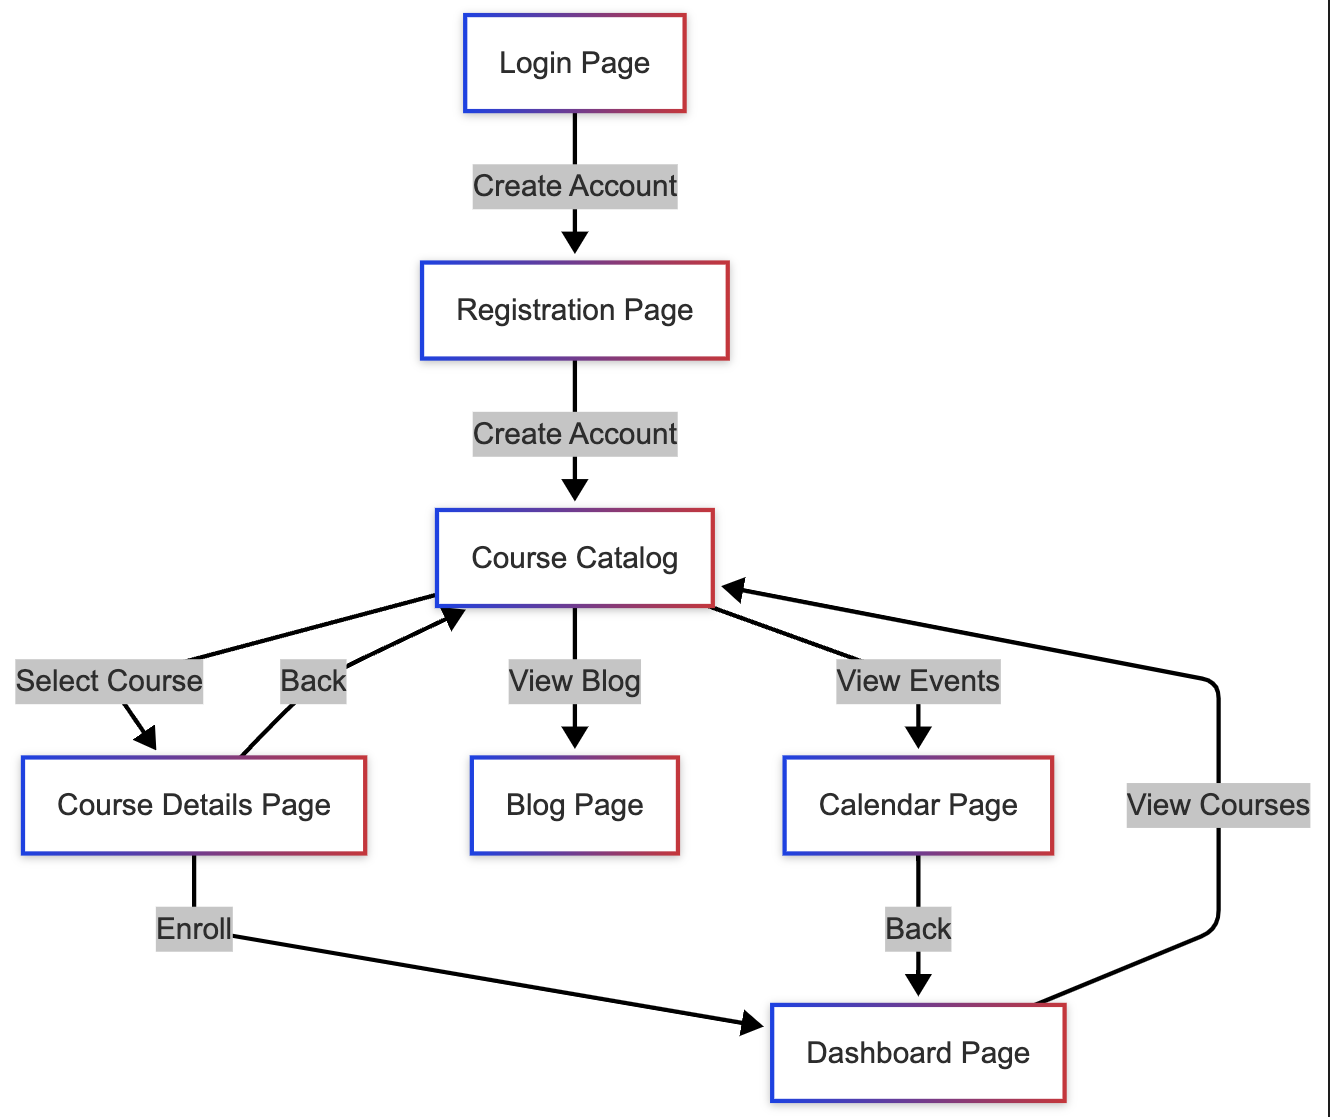
\includegraphics[width=0.9\textwidth]{UI/UI_flow.png}
%     \caption{Site Map and Navigation Flow}
% \end{figure}

\section{User-wise Navigation Flow}

\subsection{Student}
\begin{figure}[!htb]
    \centering
    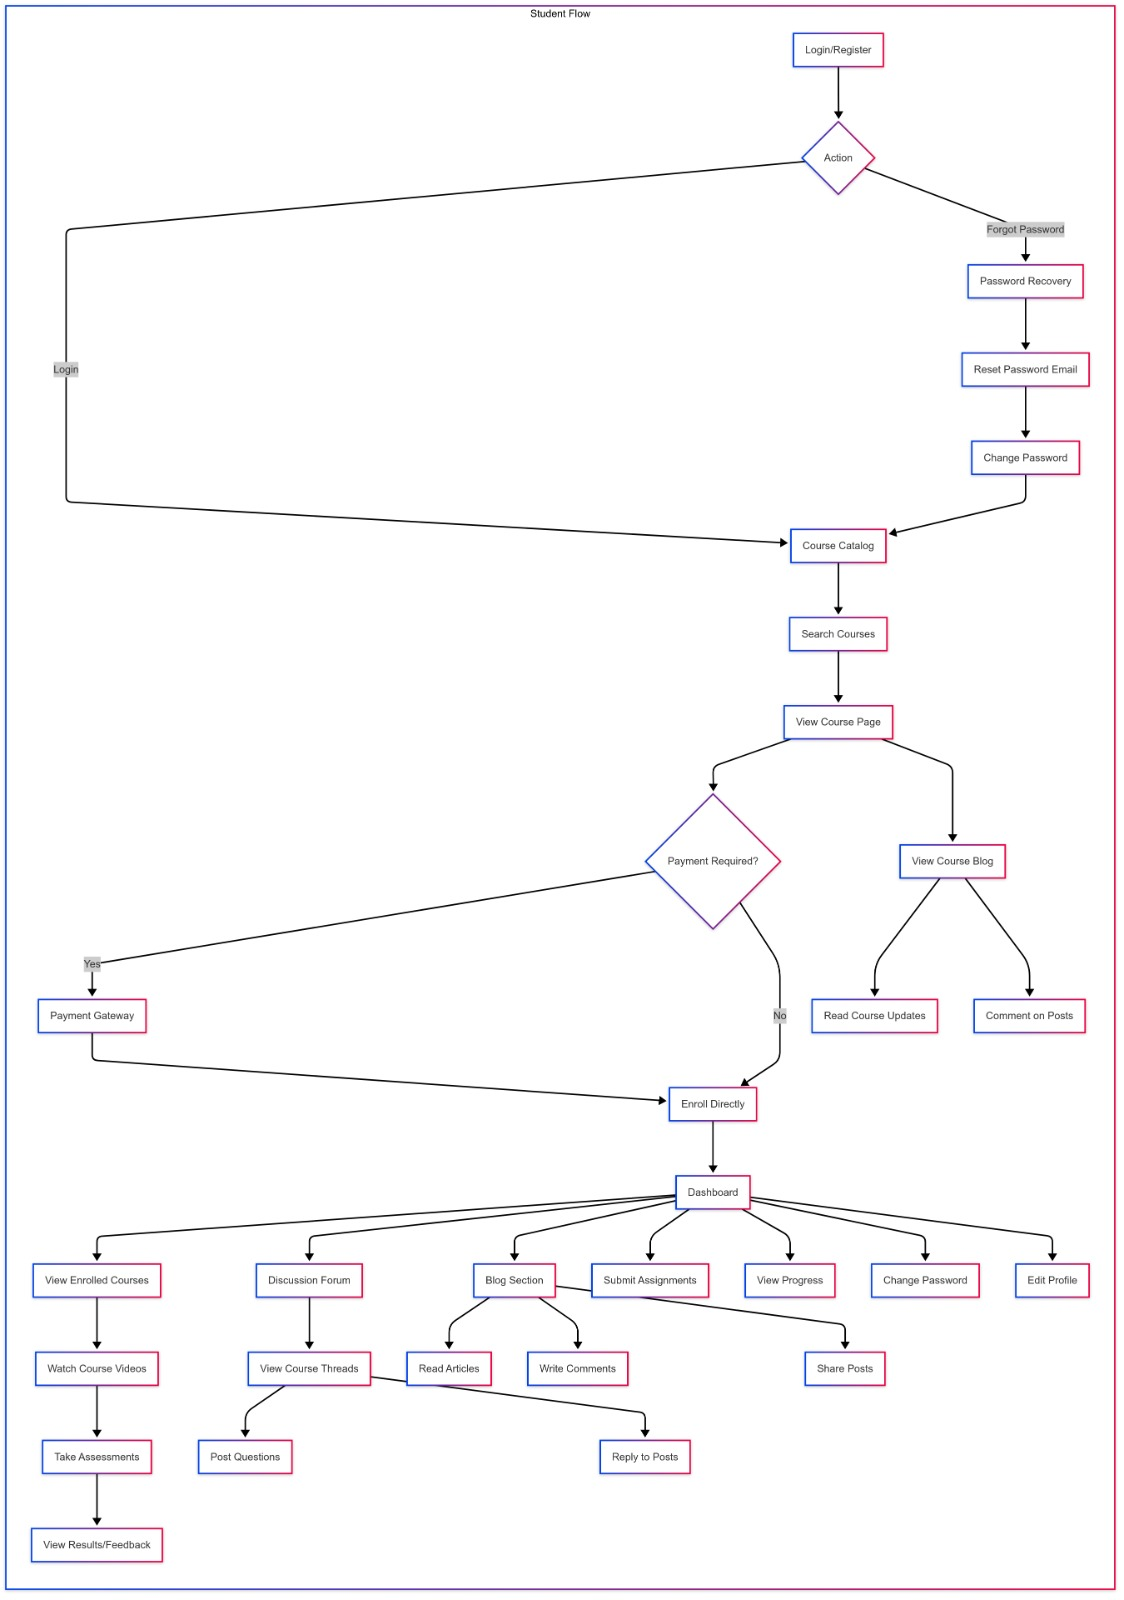
\includegraphics[height=0.63\textheight]{UI/stuFlow.jpg}
    \caption{Student Navigation Flow}
\end{figure}

\subsection{Educator}
\begin{figure}[!htb]
    \centering
    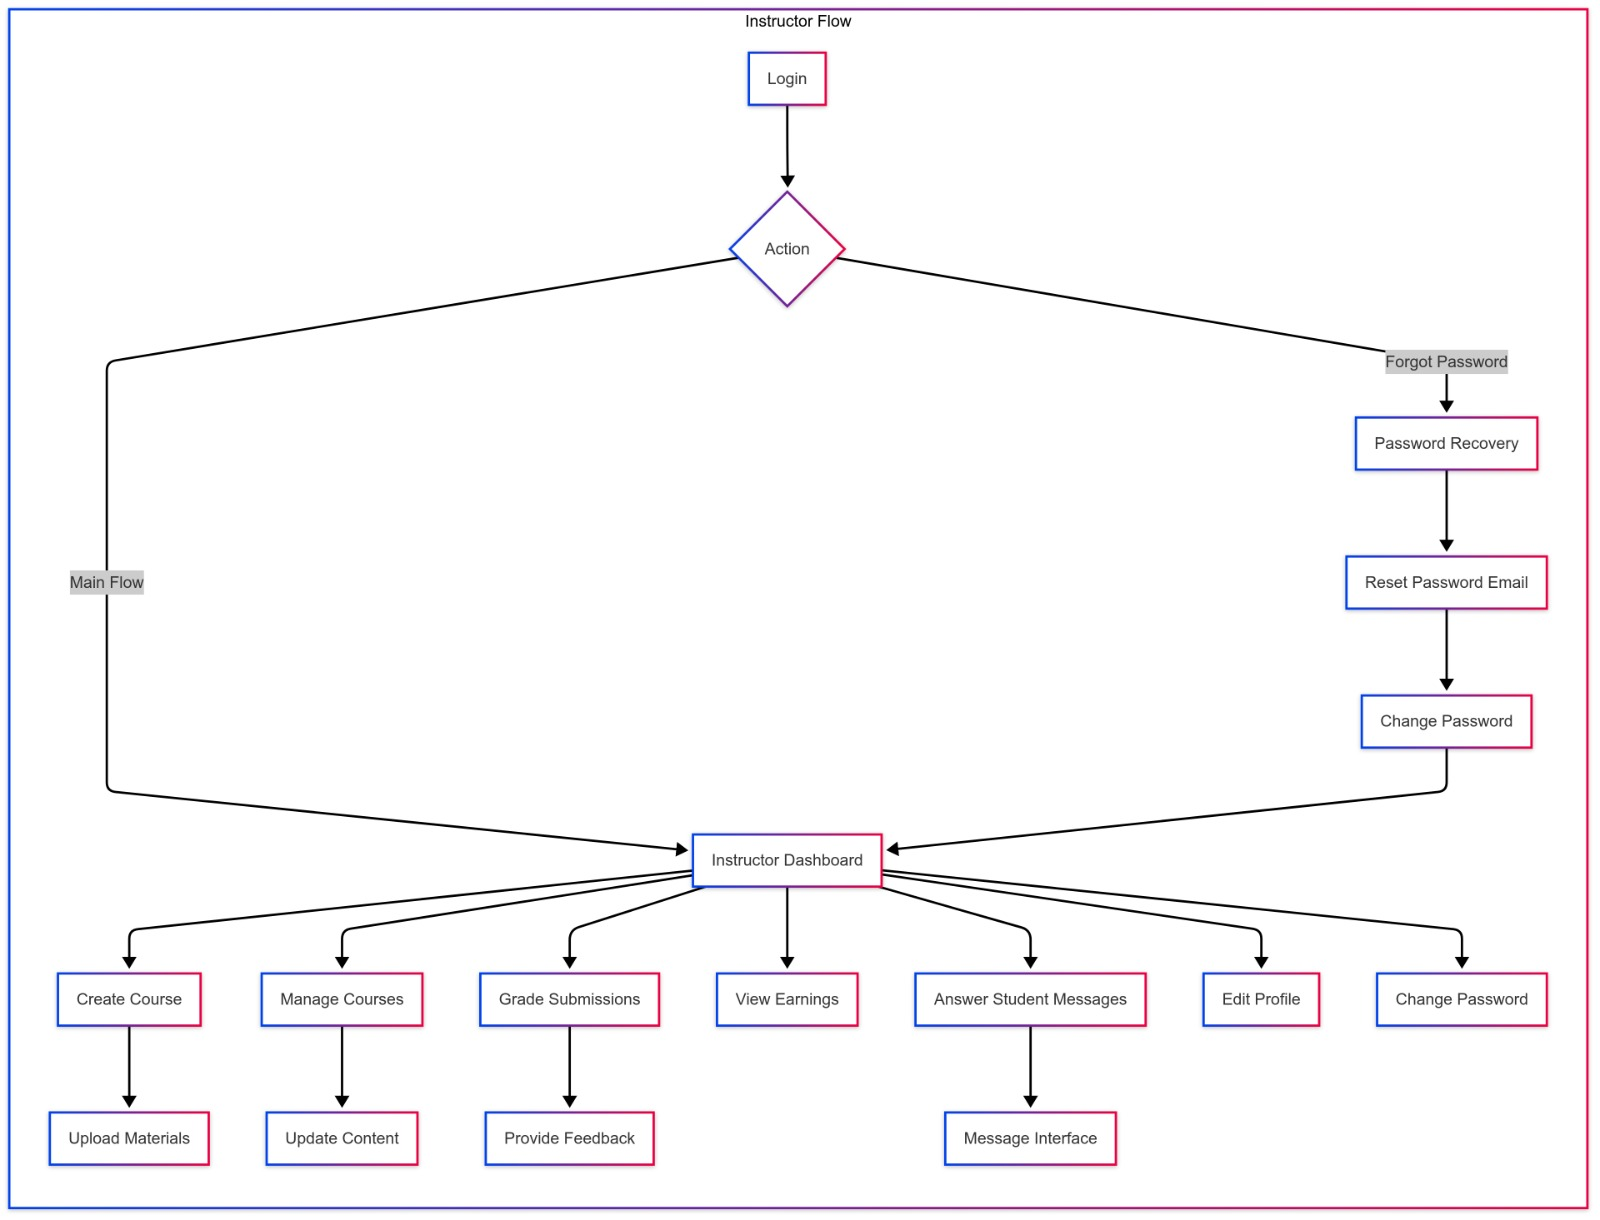
\includegraphics[height=0.3\textheight]{UI/eduFlow.jpg}
    \caption{Educator Navigation Flow}
\end{figure}

\subsection{Moderator}
\begin{figure}[!htb]
    \centering
    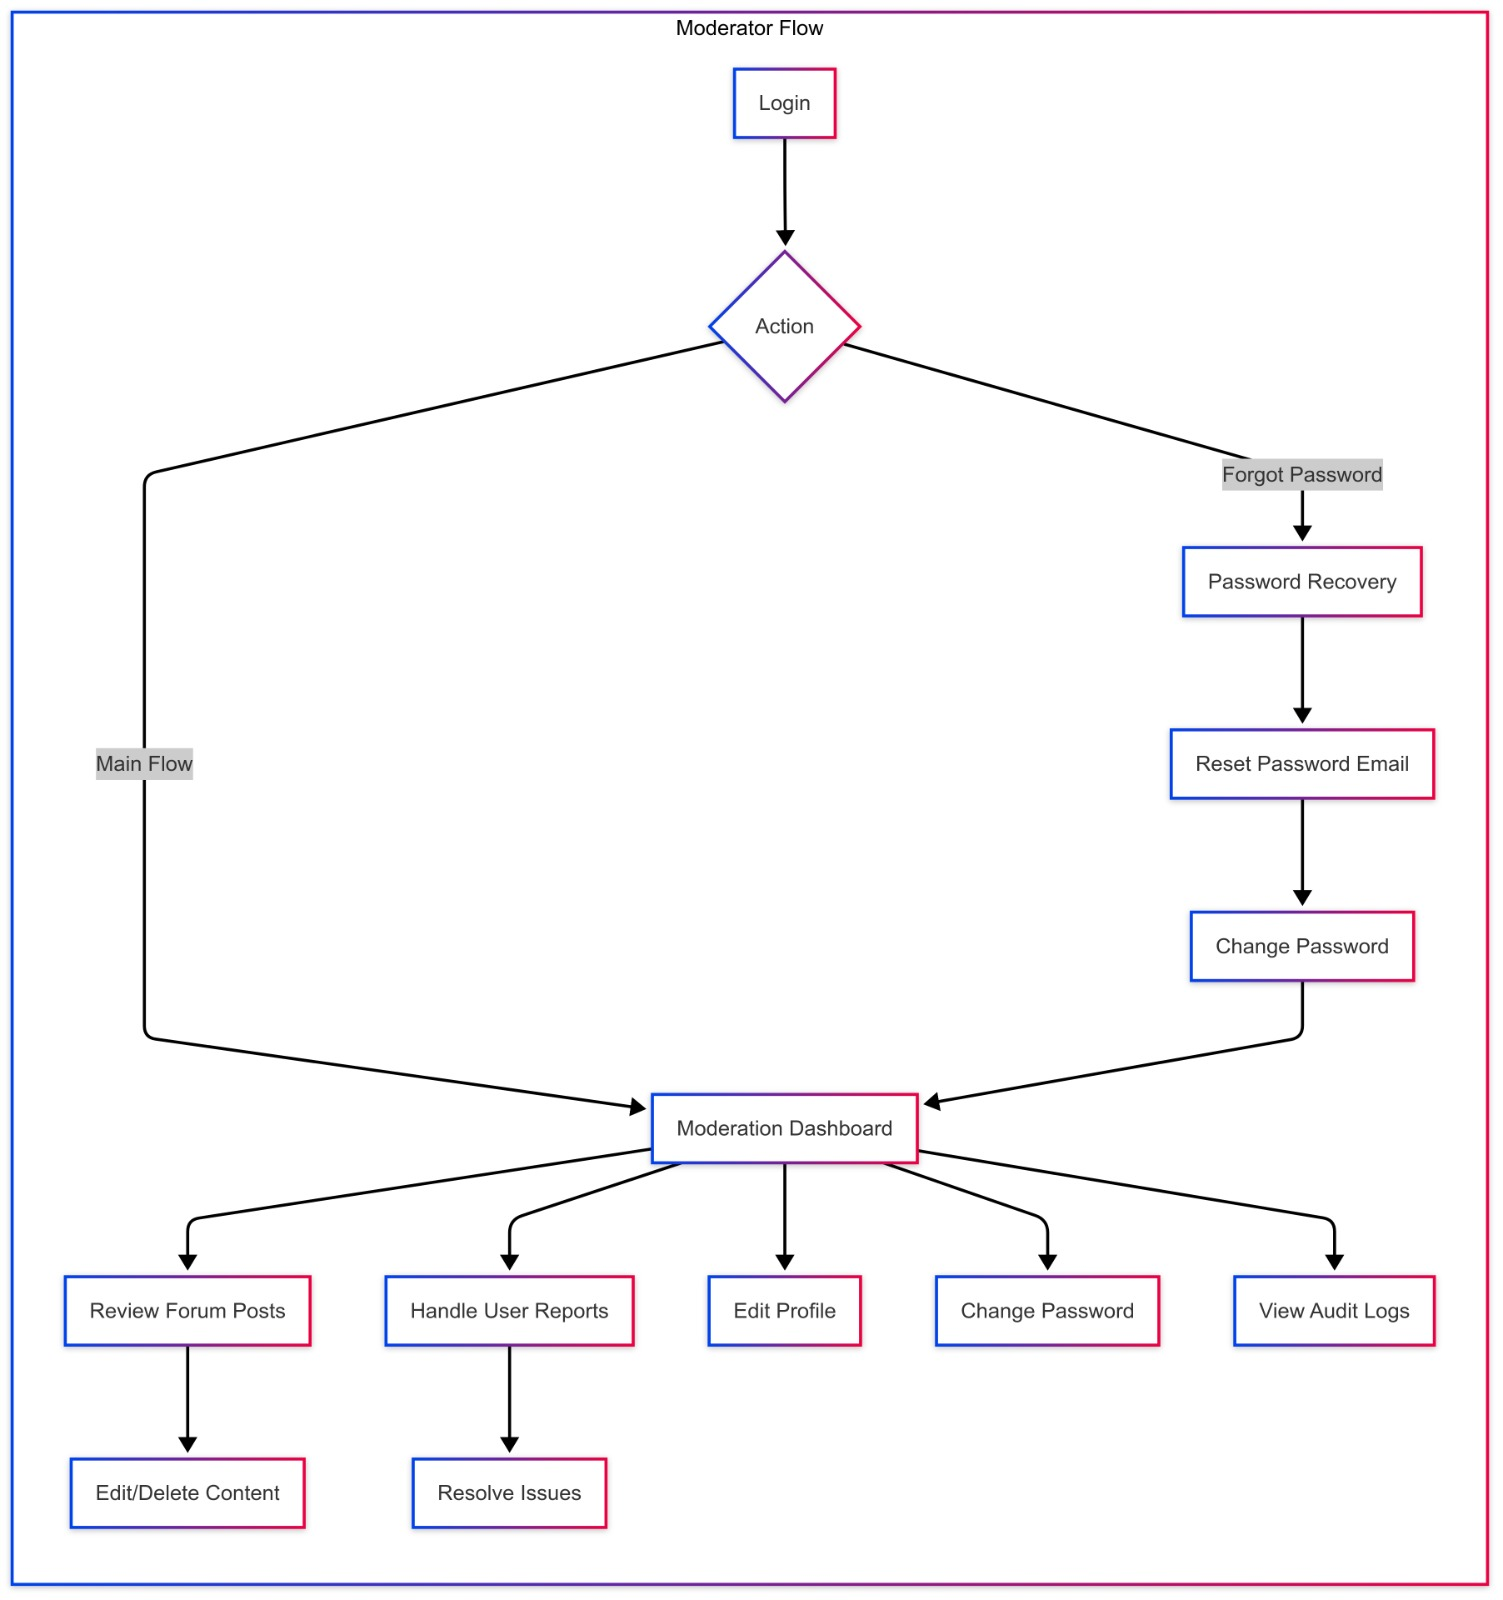
\includegraphics[height=0.5\textheight]{UI/modFlow.jpg}
    \caption{Moderator Navigation Flow}
\end{figure}

\section{Interface Storyboards}
This section showcases the key user interface screens and their relationships, depicting the actual flow of user interactions within the application.

\subsection{Authentication Flow}
\begin{figure}[ht]
    \centering
    \begin{subfigure}[b]{0.45\textwidth}
        \centering
        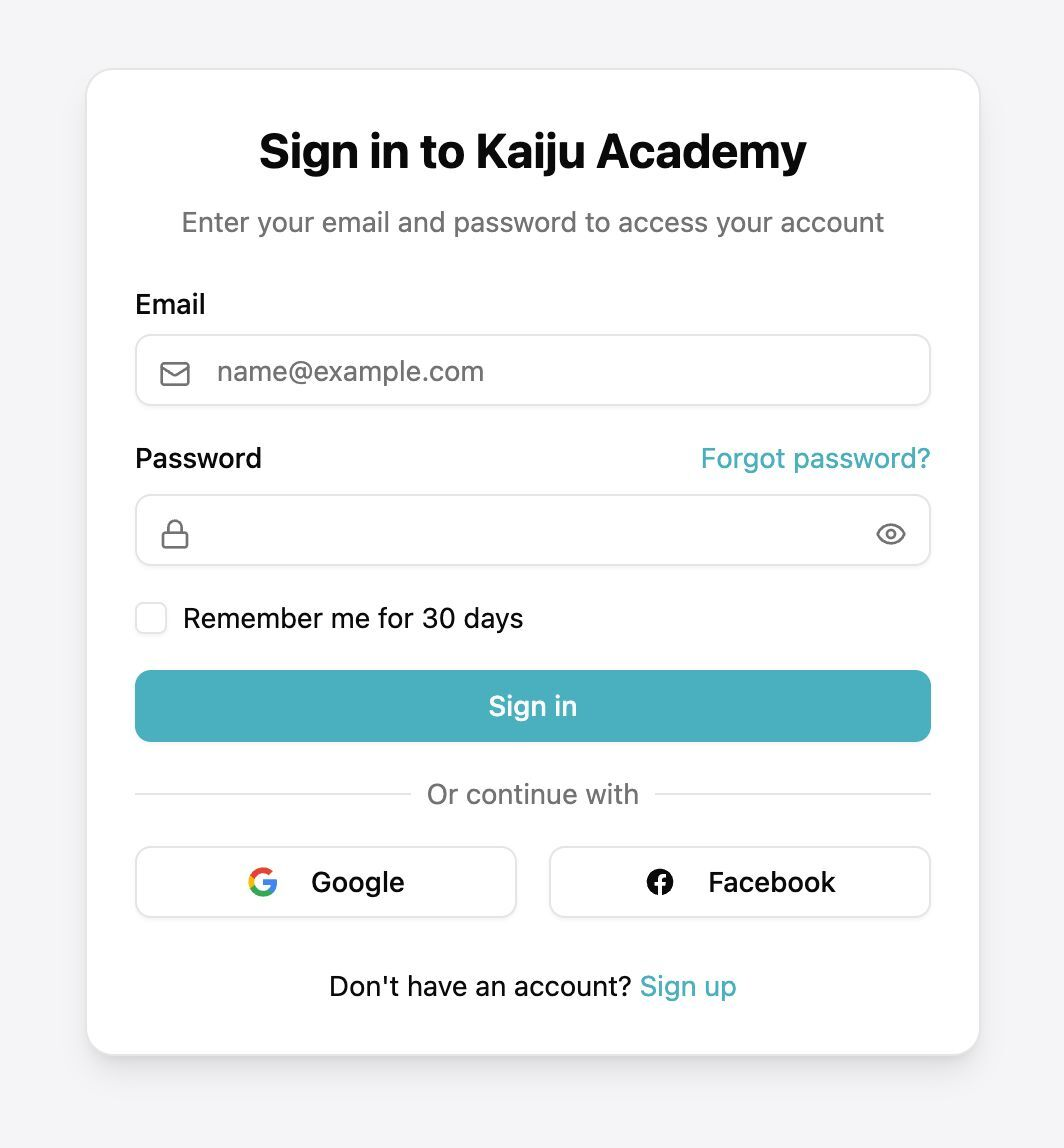
\includegraphics[width=\textwidth]{UI/SignIn.jpg}
        \caption{Sign In Screen}
    \end{subfigure}
    \hfill
    \begin{subfigure}[b]{0.45\textwidth}
        \centering
        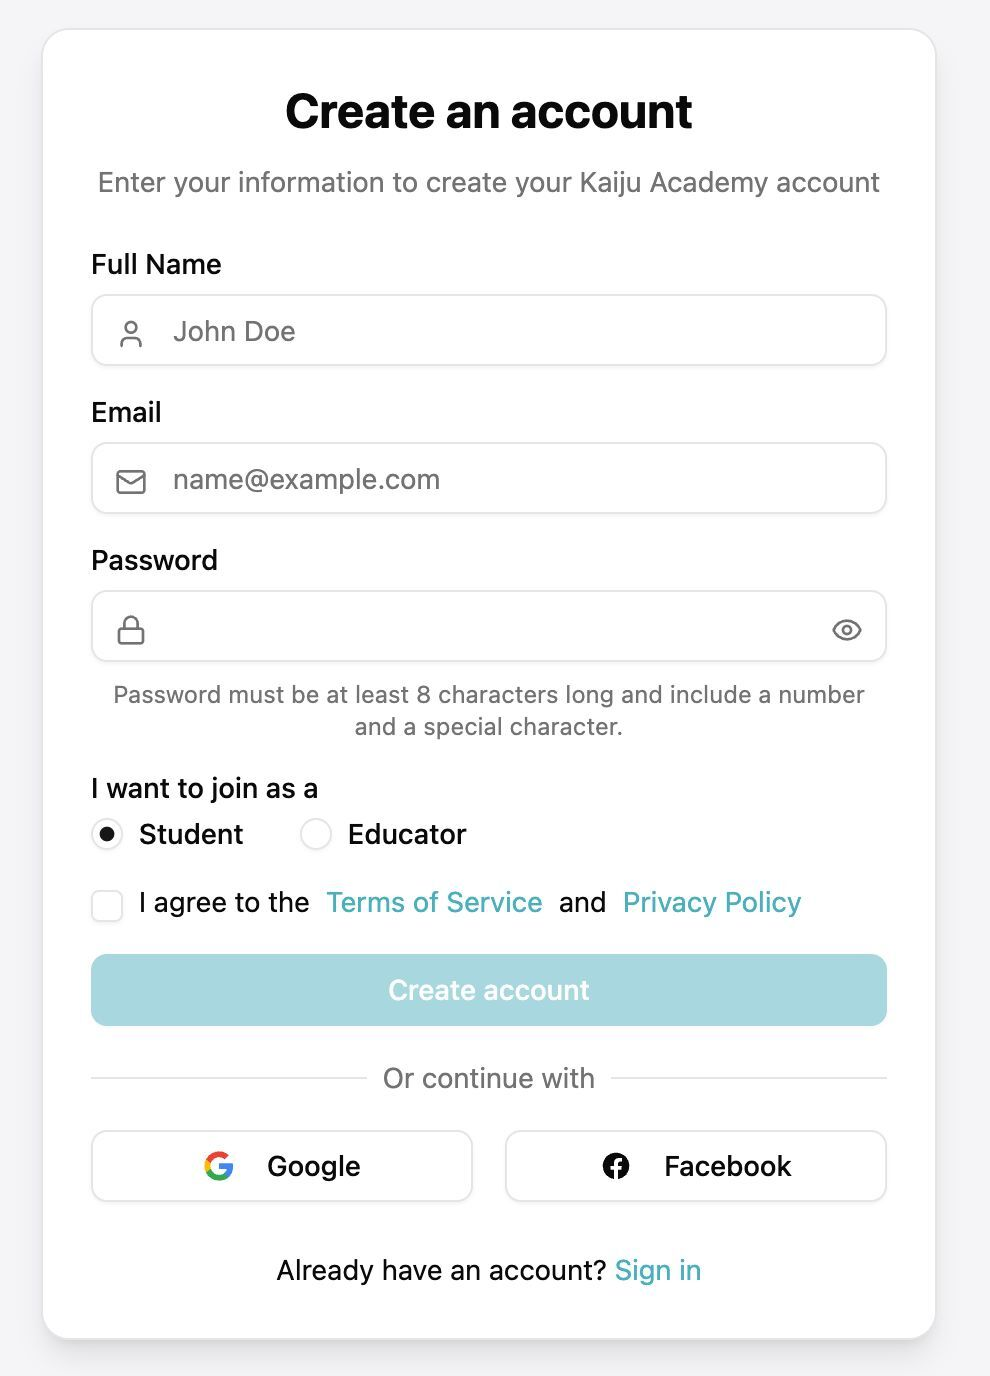
\includegraphics[width=\textwidth]{UI/SignUp.jpg}
        \caption{Sign Up Screen}
    \end{subfigure}
    
    \caption{Authentication Screens}
\end{figure}

\subsection{Student Learning Journey}
After login, the student will be redirected to the dashboard.
\begin{figure}[H]
    \centering
    \begin{subfigure}[b]{0.45\textwidth}
        \centering
        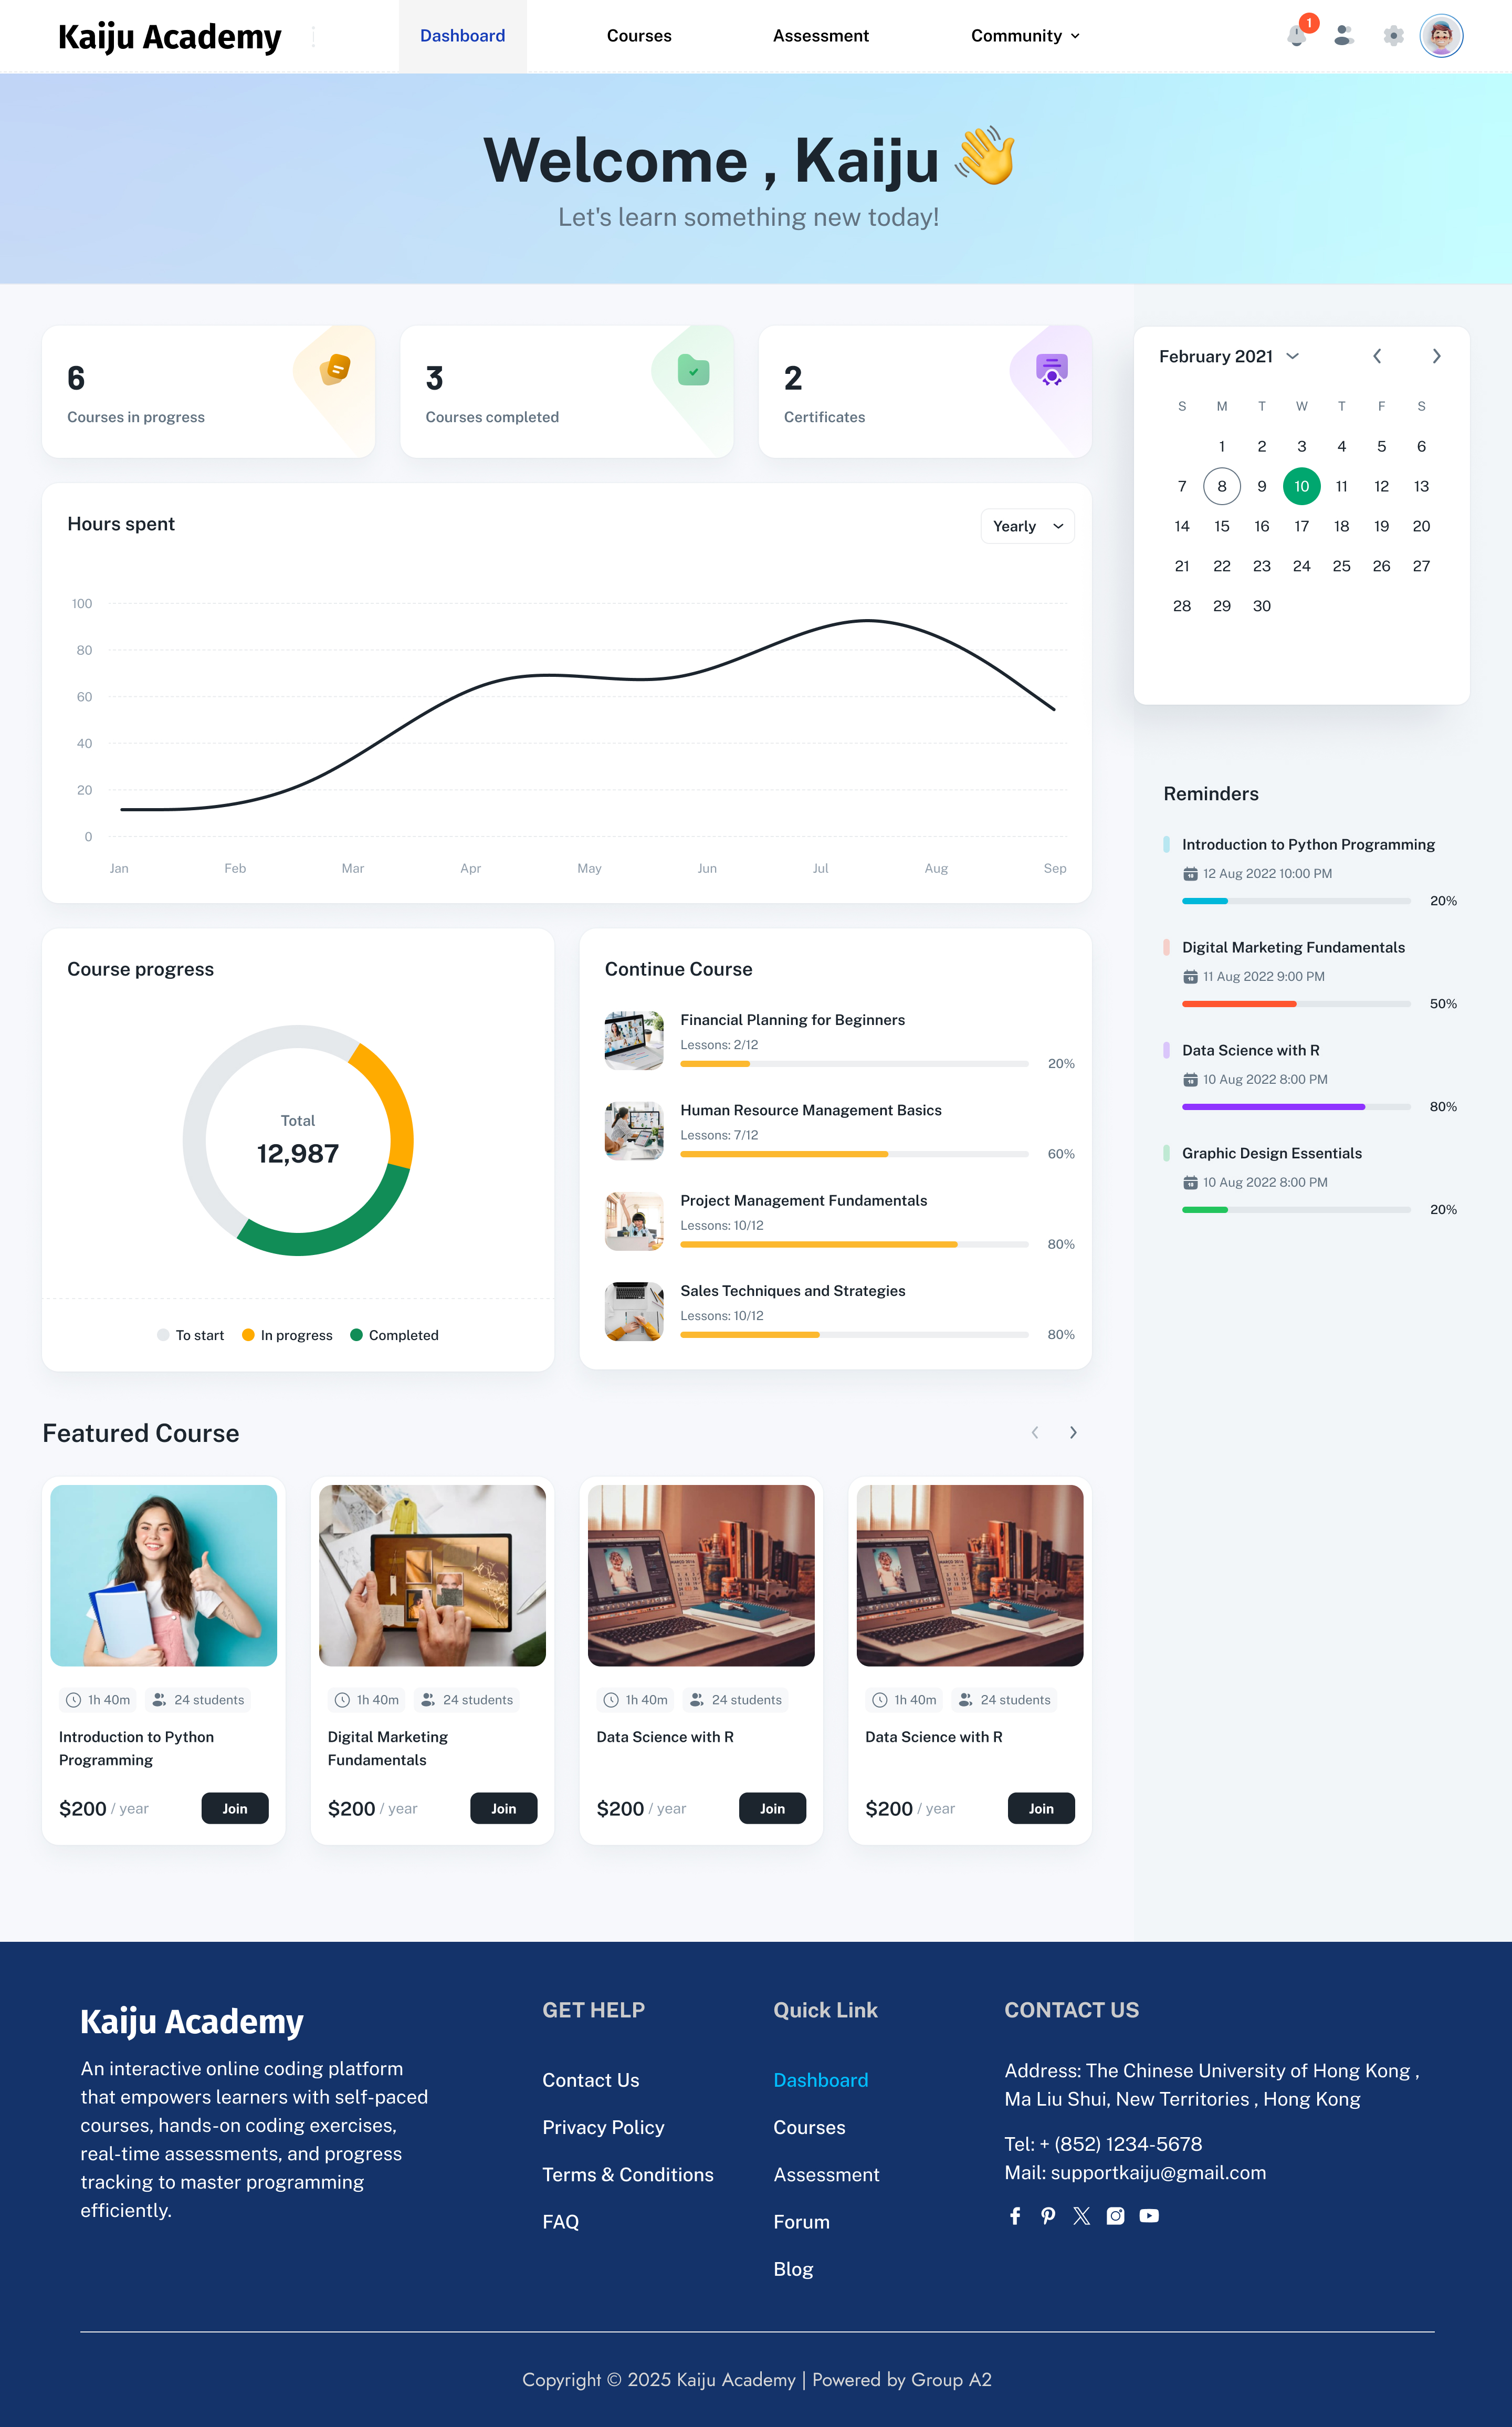
\includegraphics[height=0.4\textheight]{UI/Dashboard.jpg}
        \caption{Student Dashboard}
    \end{subfigure}
    \hfill
    \begin{subfigure}[b]{0.45\textwidth}
        \centering
        \includegraphics[height=0.4\textheight]{UI/All Courses.jpg}
        \caption{Course Catalog}
    \end{subfigure}
    \caption{Student courses view}
\end{figure}

\subsection{Learning Environment}
\begin{figure}[ht]
    \centering
    \begin{subfigure}[b]{0.32\textwidth}
        \centering
        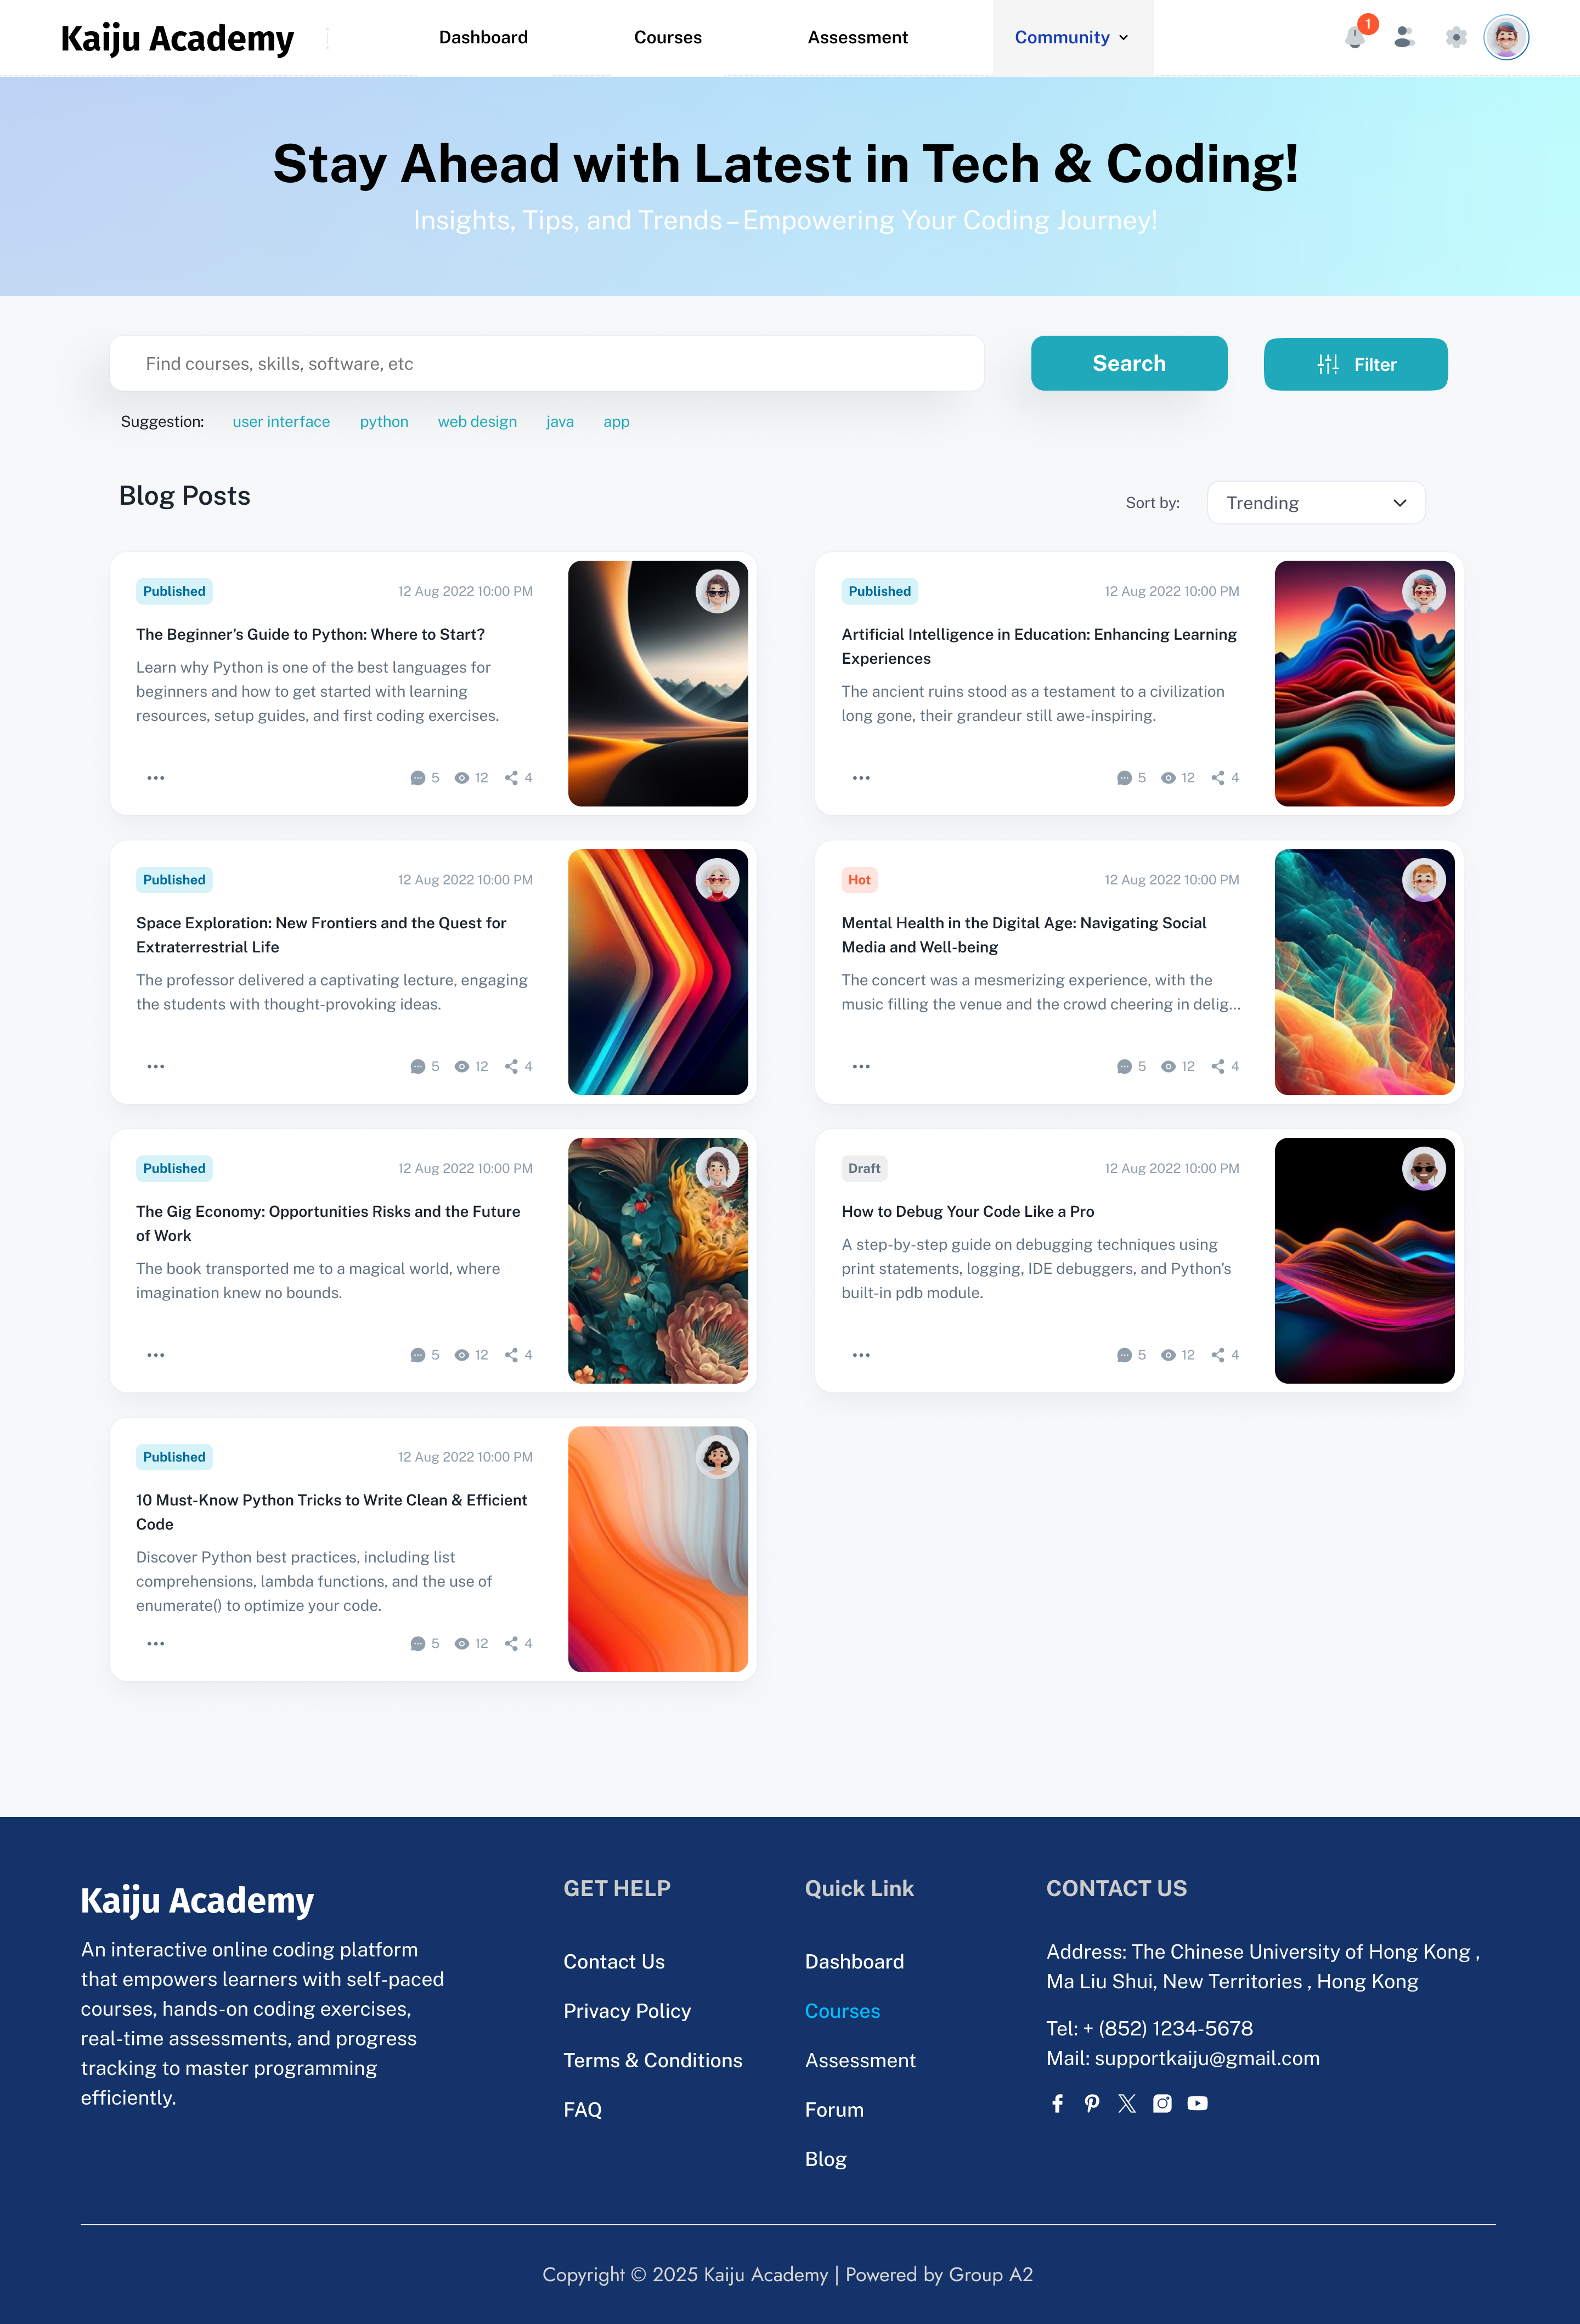
\includegraphics[width=\textwidth]{UI/Blog.jpg}
        \caption{Learning Blog}
    \end{subfigure}
    \hfill
    \begin{subfigure}[b]{0.32\textwidth}
        \centering
        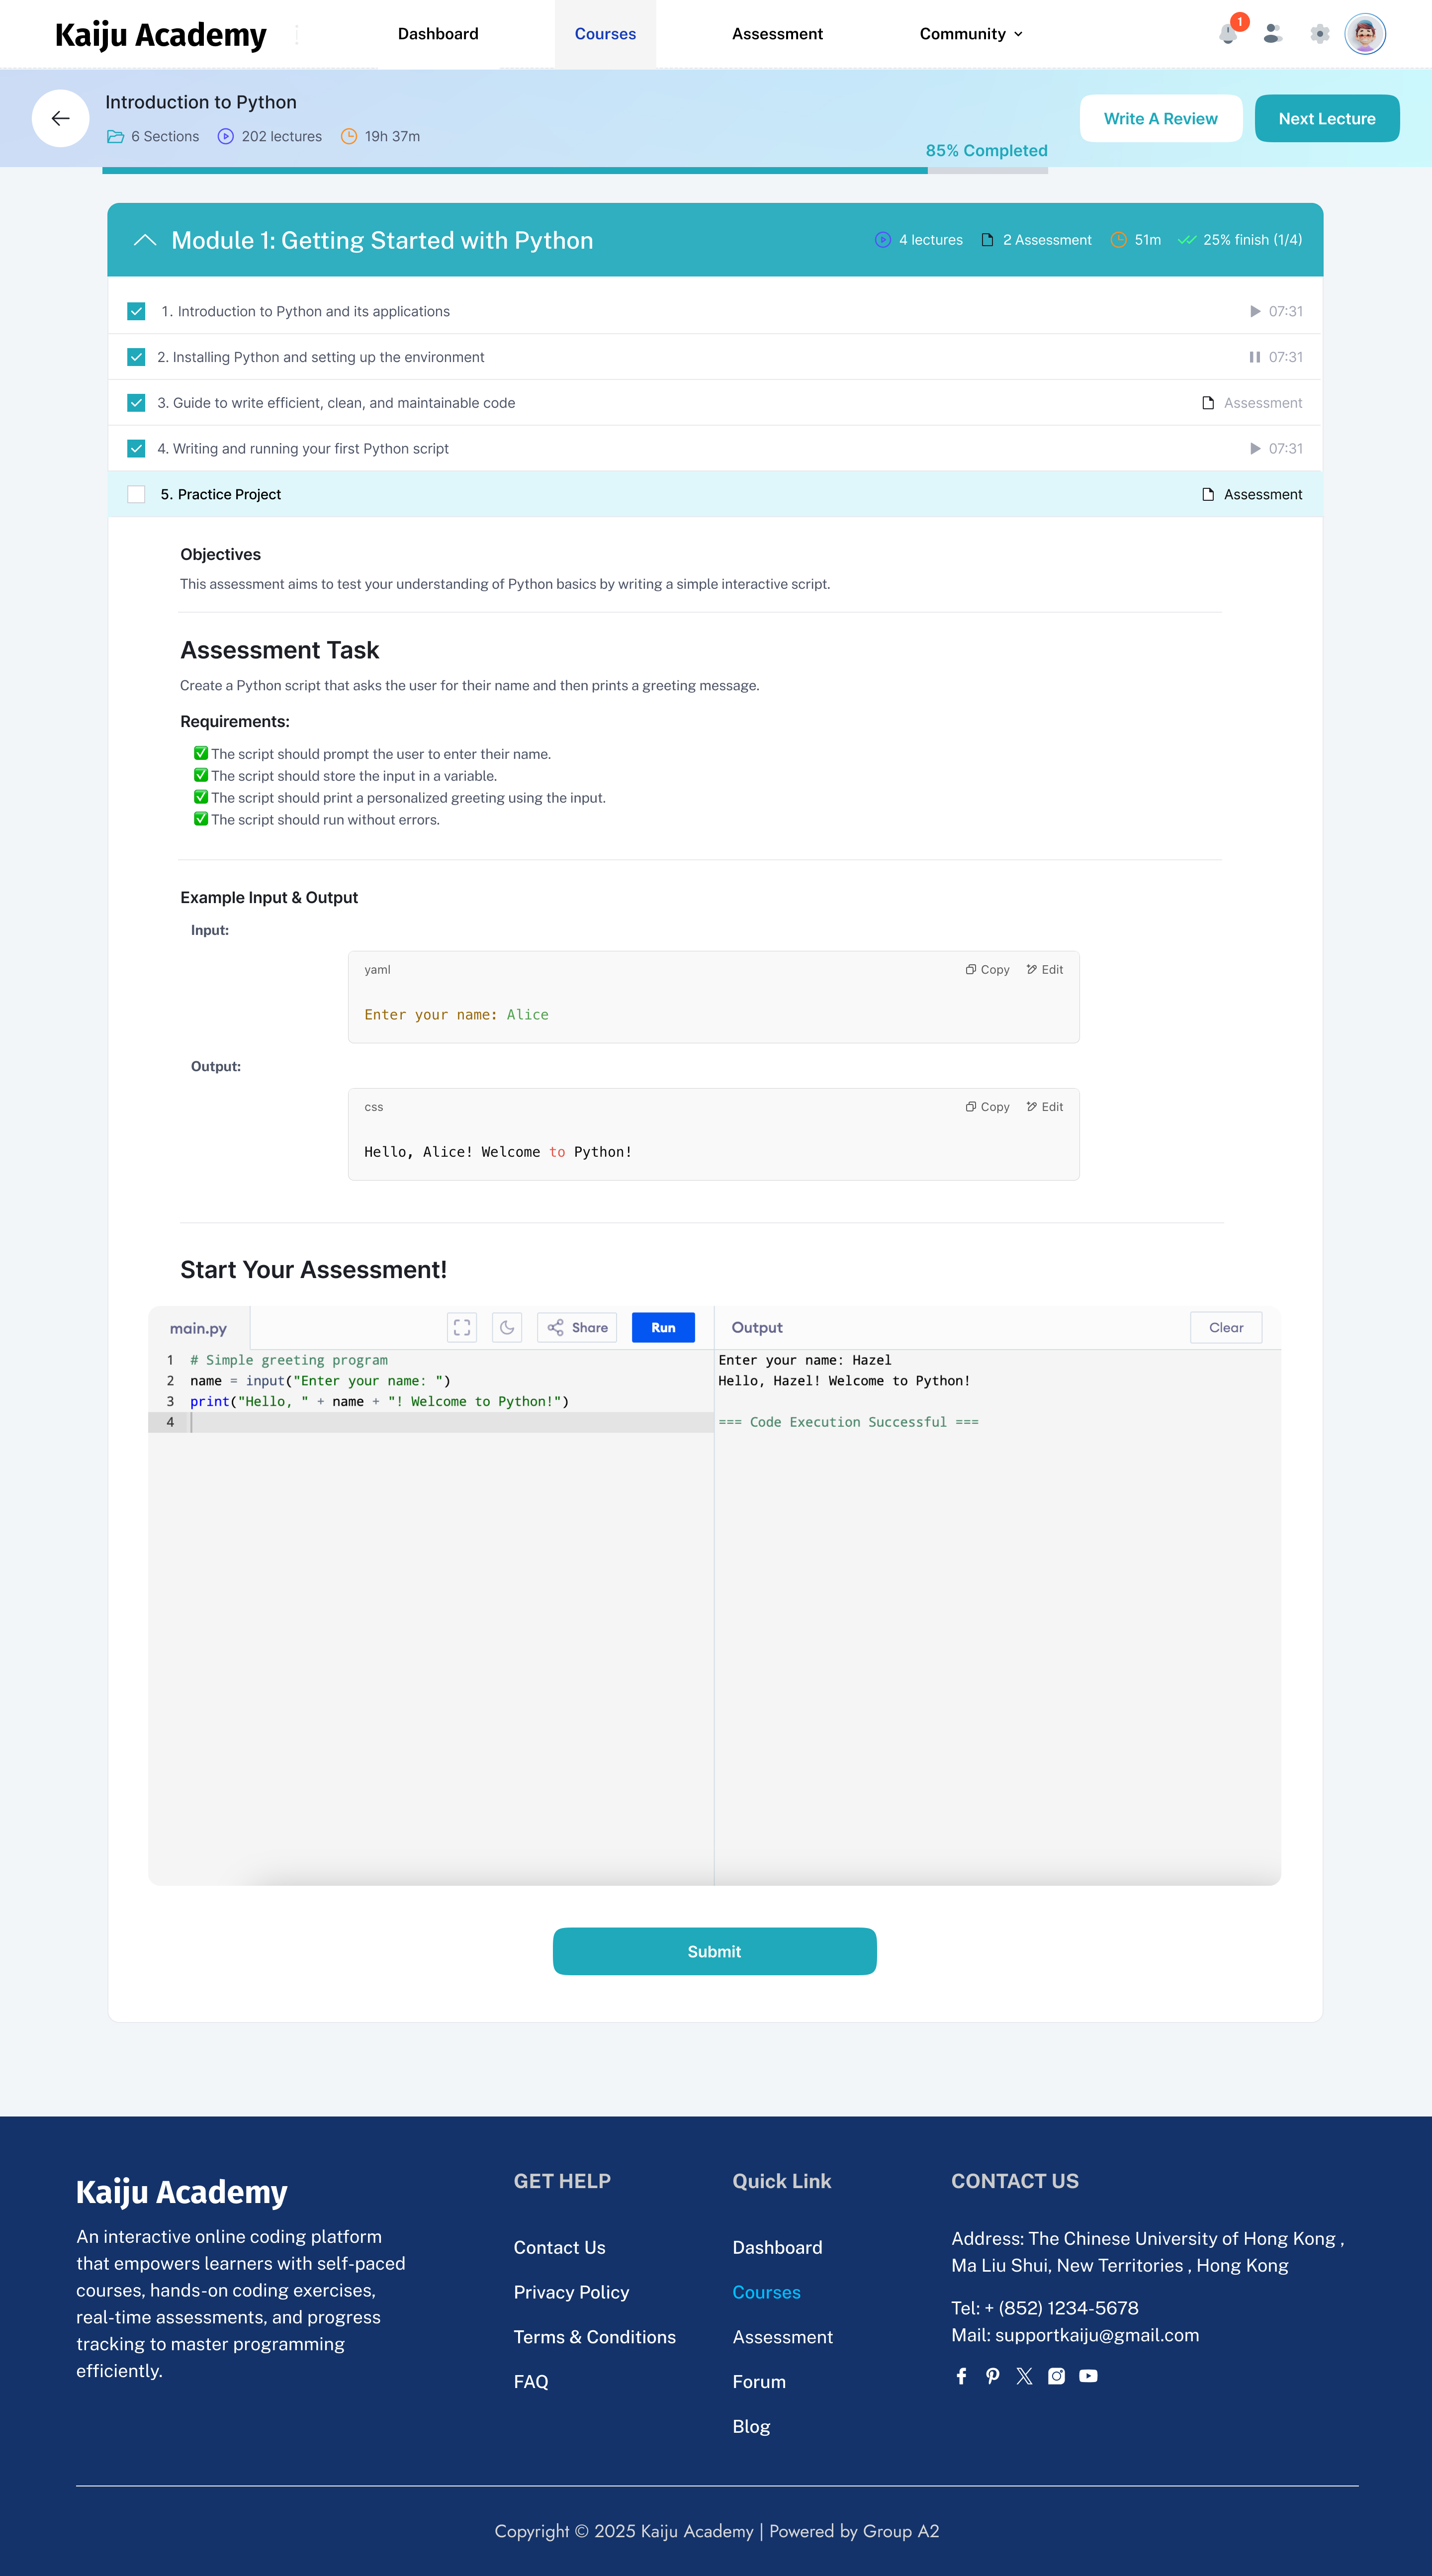
\includegraphics[width=\textwidth]{UI/Assessment.jpg}
        \caption{Assessment Interface}
    \end{subfigure}
    \hfill
    \begin{subfigure}[b]{0.32\textwidth}
        \centering
        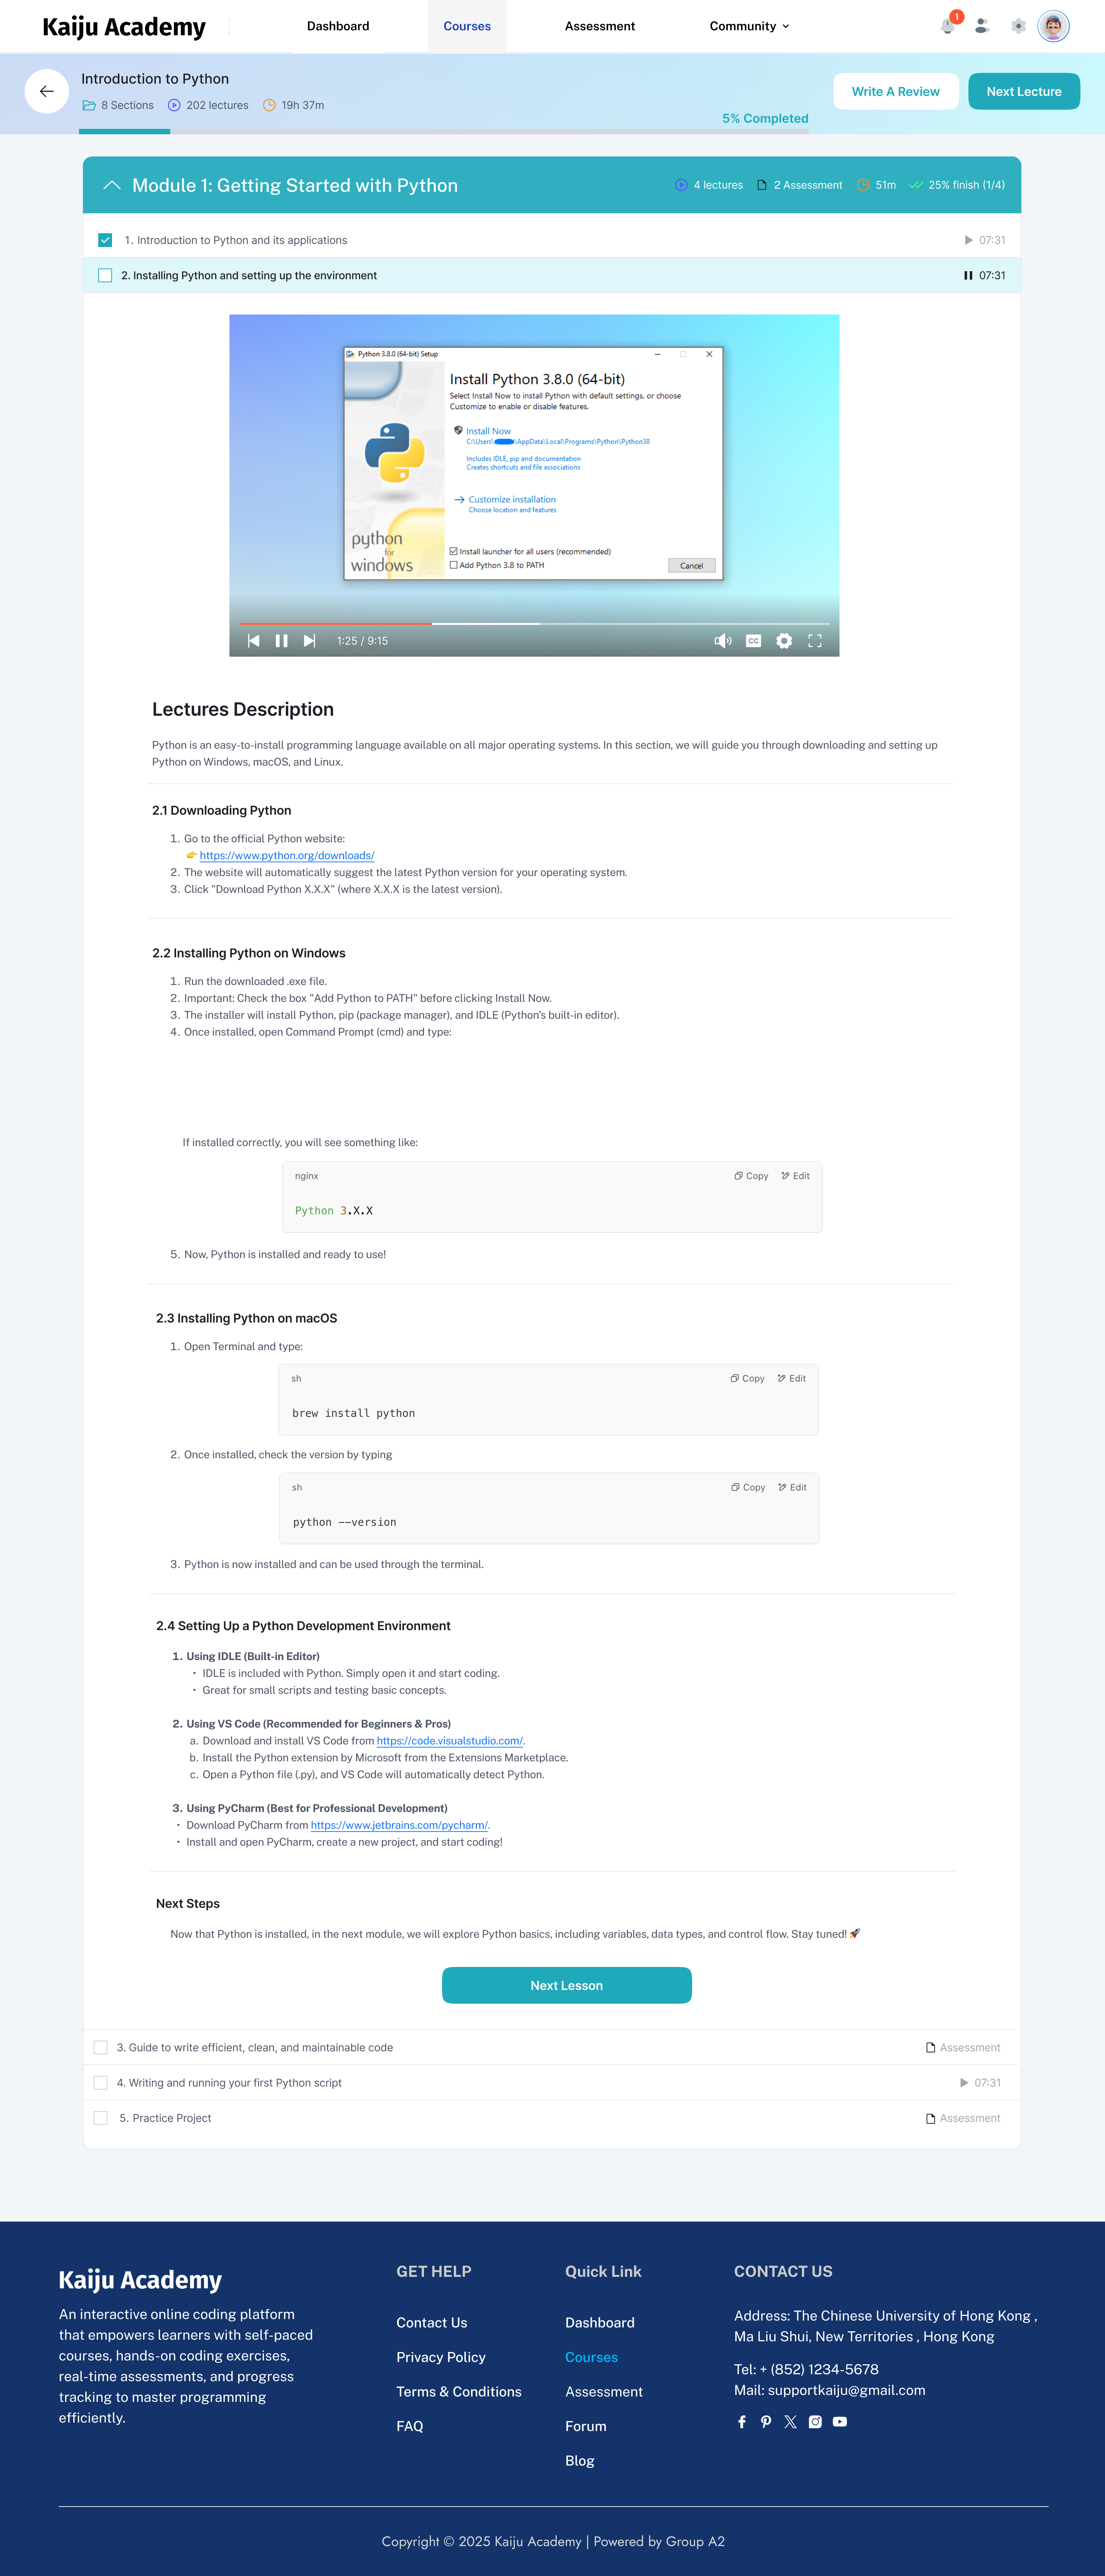
\includegraphics[width=\textwidth]{UI/During Course.jpg}
        \caption{During Course Interface}
    \end{subfigure}
    
    \caption{Learning and Assessment Interface}
\end{figure}

\section{Accessibility Considerations}
\begin{itemize}
    \item \textbf{Screen Reader Support:} Proper ARIA labels and semantic HTML
    \item \textbf{Text Resize:} Interface remains functional when text is enlarged 200\%
    \item \textbf{Motion Control:} Animations can be disabled via prefers-reduced-motion
    \item \textbf{Alternative Text:} All images include descriptive alt text
    \item \textbf{Light/Dark Mode:} Option to switch between light and dark themes for user preference
    \item \textbf{Font Size Adjustment:} Users can easily enlarge or reduce font size for better readability
    \item \textbf{Color Blindness Support:} Special color sets available to accommodate color blindness
\end{itemize}

\section{Responsive Design}
\begin{itemize}
    \item \textbf{Breakpoints:} Key breakpoints at 480px, 768px, 1024px, and 1440px
    \item \textbf{Layout Adaptations:} 
    \begin{itemize}
        \item Single column layout on mobile
        \item Sidebar appears as overlay on small screens
        \item Multi-column layout on tablets and larger
        \item Expanded dashboard visualizations on desktop
    \end{itemize}
    \item \textbf{Touch Targets:} Minimum 44$\times$44px for all interactive elements
\end{itemize}

\chapter{Assumptions}

\section{Technical Constraints}

\subsection{Hardware Constraints}
\begin{itemize}
    \item \textbf{Minimum Device Specifications:} Users require devices with:
    \begin{itemize}
        \item At least 4GB RAM for smooth performance
        \item Screen resolution of 320px width minimum
        \item Internet connection with 5 Mbps minimum bandwidth
    \end{itemize}
    
    \item \textbf{Server Environment:} Development and deployment assumes:
    \begin{itemize}
        \item AWS cloud infrastructure
        \item Serverless architecture with AWS Lambda
        \item No dedicated hardware requirements
        \item Horizontal scaling capabilities
    \end{itemize}
\end{itemize}

\subsection{Software Constraints}
\begin{itemize}
    \item \textbf{Browser Support:} Application designed for:
    \begin{itemize}
        \item Modern browsers (Chrome, Firefox, Safari, Edge - latest 2 versions)
        \item HTML5 and JavaScript required
    \end{itemize}
    
    \item \textbf{Mobile Support:}
    \begin{itemize}
        \item Responsive web design (no native app initially)
        \item Mobile browser focused (iOS Safari, Android Chrome)
    \end{itemize}
\end{itemize}

\section{Operational Assumptions}

\subsection{Load and Performance}
\begin{itemize}
    \item Peak submission rate: 10,000 code submissions per minute
    \item 80/20 read/write ratio for database operations
    \item Code execution takes maximum 5 seconds per submission
\end{itemize}

\subsection{Development Process}
\begin{itemize}
    \item CI/CD pipeline with automated testing
    \item Feature branching development workflow
\end{itemize}

\subsection{Maintenance and Support}
\begin{itemize}
    \item 99.9\% uptime requirement excluding planned maintenance
    \item Automated backups performed daily and retained for 30 days
\end{itemize}

\section{Dependencies}

\subsection{Third-Party Services}
\begin{itemize}
    \item Authentication via OAuth providers (Google, GitHub, Microsoft)
    \item Payment processing through Stripe
    \item Email delivery through Amazon SNS
    \item CDN services through AWS CloudFront
    \item Media transcoding through AWS MediaConvert
\end{itemize}

\end{document} 